% document's head

\begin{center}
    \LARGE \textsc{Название}
\end{center}

\hrule

\phantom{42}

\begin{flushright}
    \begin{tabular}{rr}
    % written by:
        % \textbf{Источник}: 
        % & \href{__ссылка__}{__название__} \\
        % & \\
        % \textbf{Лектор}: 
        % & _ФИО_ \\
        % & \\
        \textbf{Авторы заметок}: 
        & Хоружий Кирилл \\
        % & Примак Евгений \\
        & \\
    % date:
        \textbf{От}: &
        \textit{\today}\\
    \end{tabular}
\end{flushright}

\thispagestyle{empty}
\tableofcontents
\newpage


% \section*{Exercises and tasks}


\addcontentsline{toc}{section}{Exercises and tasks}


\addcontentsline{toc}{subsection}{1.1 \ \ Equations of motion for creation and annihilation operators}
\addcontentsline{toc}{subsection}{1.2 \ \ Non-interacting lattice fermions}
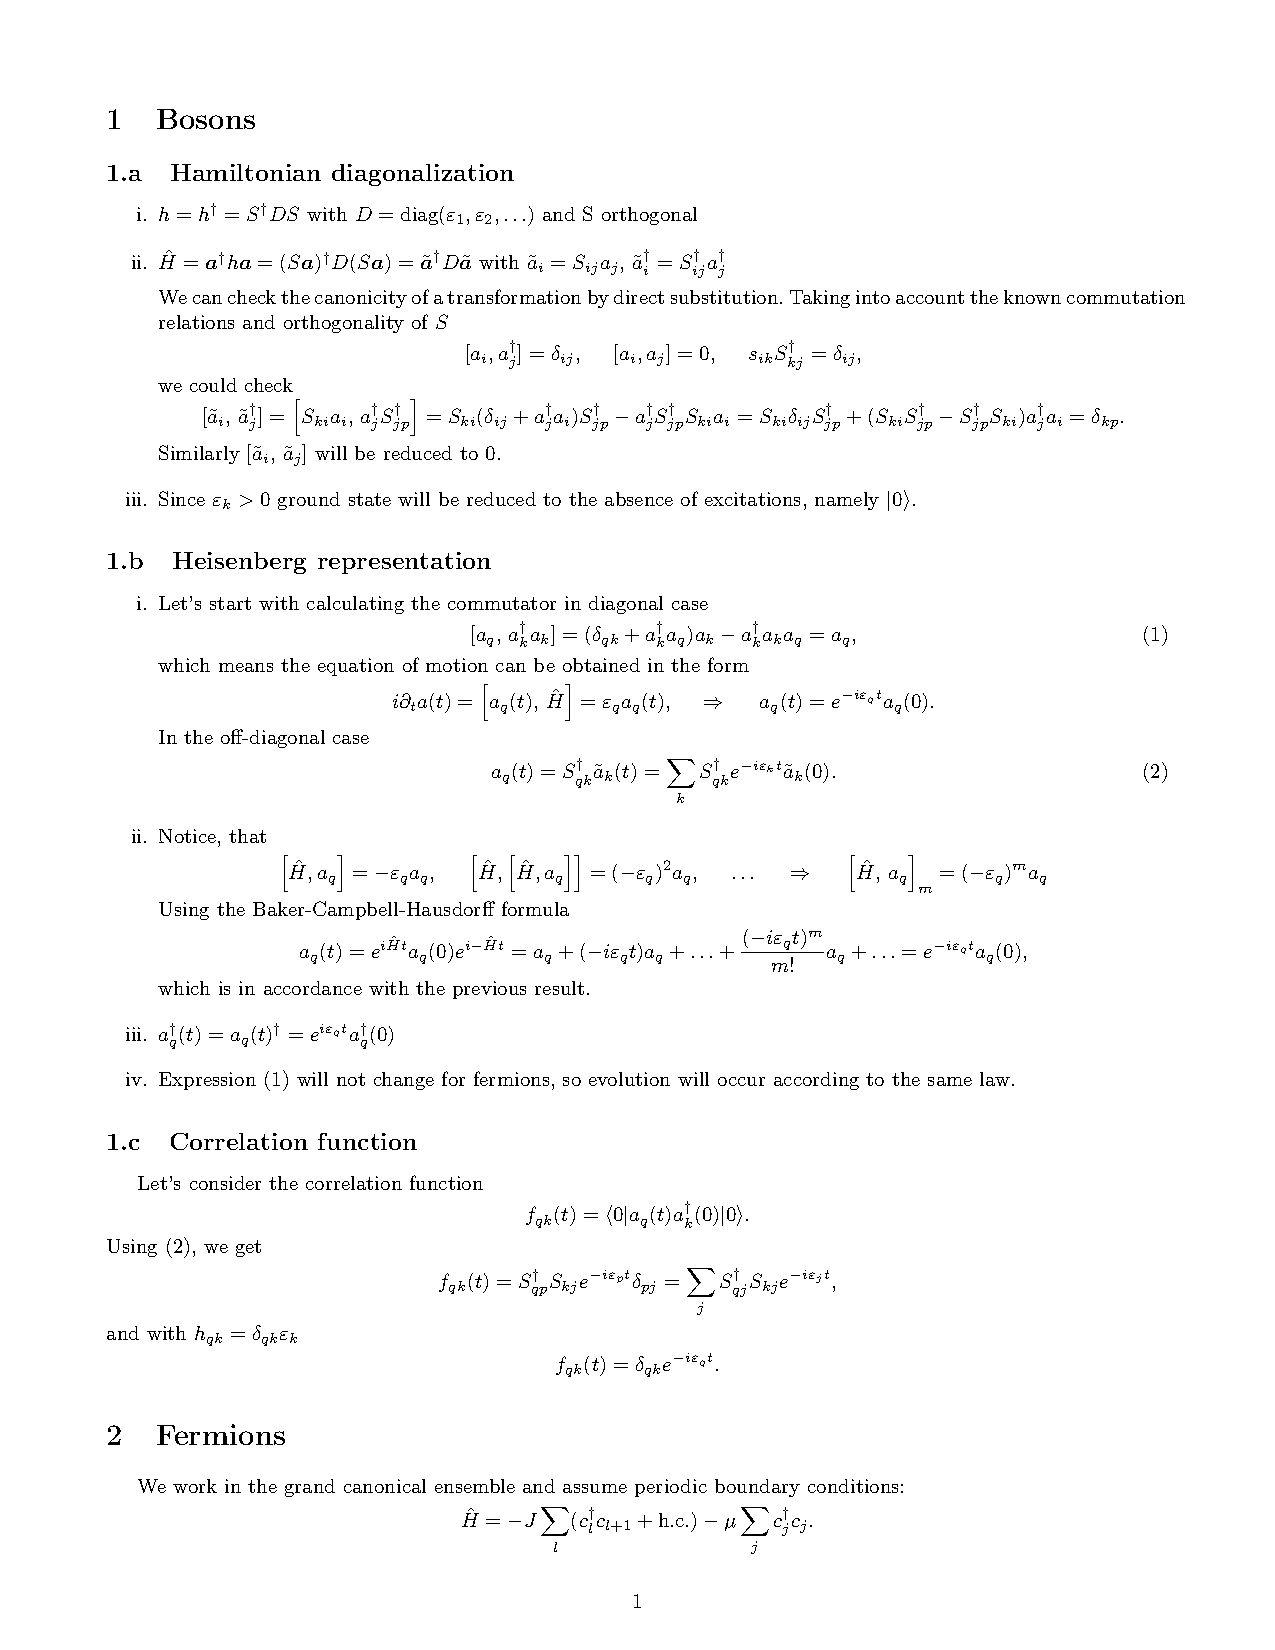
\includepdf[pages=-]{MBs1.pdf}

% % Lorem ipsum dolor sit amet, consectetur adipisicing elit, sed do eiusmod
% tempor incididunt ut labore et dolore magna aliqua. Ut enim ad minim veniam,
% quis nostrud exercitation ullamco laboris nisi ut aliquip ex ea commodo
% consequat. Duis aute irure dolor in reprehenderit in voluptate velit esse
% cillum dolore eu fugiat nulla pariatur. Excepteur sint occaecat cupidatat non
% proident, sunt in culpa qui officia deserunt mollit anim id est laborum.
% \begin{equation*}
% 	\ket{\psi} = \alpha_1 \raisebox{-6.3mm}{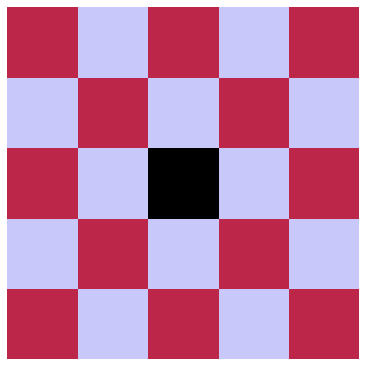
\includegraphics[width=0.08\textwidth]{s1.pdf}} + 
% 	\alpha_2 \raisebox{-6.3mm}{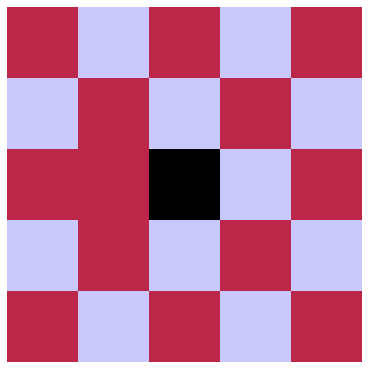
\includegraphics[width=0.08\textwidth]{s2.pdf}} + 
% 	\alpha_3 \raisebox{-6.3mm}{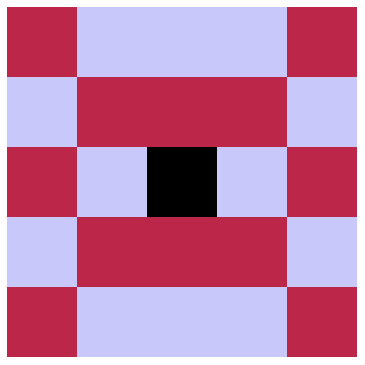
\includegraphics[width=0.08\textwidth]{s3.pdf}} + \ldots
% \end{equation*}

% \begin{equation*}
% 	\hat{H} = J \sum_{\langle i,j\rangle} \hat{S}_i \hat{S}_j - t \sum_{\langle i,j\rangle} \hat{c}_i\D \hat{c}_j
% \end{equation*}

% \begin{equation*}
% 	f(z) = \left\{\begin{aligned}
% 	    &1 - {\tilde{N}^0_{\text{pred}> z}}/{\tilde{N}^1_{\text{pred}< z}}, &z \geq \text{treshold} \\
% 	    &{\tilde{N}^1_{\text{pred}< z}}/{\tilde{N}^0_{\text{pred}> z}}-1, &z < \text{treshold} \\
% 	\end{aligned}\right.
% \end{equation*}


% \begin{equation*}
% 	f(z) = \tilde{N}^1_{\text{pred}< z}
% \end{equation*}


%  \begin{equation*}
%  	\hat{H} = - \sum_{\langle i,j\rangle} \hat{c}_i\D \hat{c}_j
%  \end{equation*}

%  \begin{equation*}
%  	g_2(r) = \langle \hat{c}_{\vc{j}}\D \hat{c}_{\vc{j}+\vc{r}}\D \hat{c}_{\vc{j}+\vc{r}}\hat{c}_{\vc{j}}\rangle_{\vc{j}}
%  \end{equation*}

%  \begin{equation*}
%  	\sub{\hat{H}}{FH} = - t \sum_{\langle i,j\rangle, \sigma} \hat{c}_{i \sigma}\D \hat{c}_{j \sigma} + U \sum_j \hat{n}_{j \uparrow} \hat{n}_{j \downarrow} + \sum_{j, \sigma} (V_j - \mu)\hat{n}_{j, \sigma}
%  \end{equation*}

%  \begin{equation*}
%  	{\hat{H}}_{tJ} = - t \sum_{\langle i,j\rangle, \sigma} \hat{c}_{i \sigma}\D \hat{c}_{j \sigma} + J \sum_{\langle i,j\rangle}\left(
%  		\hat{S}_i \hat{S}_j - \tfrac{1}{4} n_i n_j
%  	\right) + O(t^3 / U^2)
%  \end{equation*}

%  \begin{equation*}
%  	\langle \hat{O}\rangle(T) = \tfrac{1}{Z}\sum_j e^{- E_j / T} \bk{\psi_j}[\hat{O}]{\psi_j}
%  \end{equation*}

% \begin{equation*}
% {\hat{H}}_{tJ} = - t \sum_{\langle i,j\rangle, \sigma} \hat{c}_{i \sigma}\D \hat{c}_{j \sigma} + J \sum_{\langle i,j\rangle}
% 	\hat{S}_i \hat{S}_j
% \end{equation*}

% Stern-Gerlach: $F = \mu_z  \cdot \tfrac{\partial B}{\partial z} $



% \begin{equation*}
% 	\begin{pmatrix}
% 		\text{cost}_1 \\ \ldots \\ \text{cost}_n
% 	\end{pmatrix} \to \begin{pmatrix}
% 		w_1 \cdot \text{cost}_1 \\ \ldots \\ w_n \cdot  \text{cost}_n
% 	\end{pmatrix} 
% \end{equation*}



\setcounter{section}{2}
\setcounter{subsection}{0}
\subsection{Second Quantization}


We could consider
\begin{equation*}
	\ket{\alpha_1,\ldots,\alpha_N} = \frac{1}{\sqrt{N!}} \sum_{P} \zeta^{\sigma(P)} 
	\ket{\alpha_{P(1)}} \otimes \ldots \otimes \ket{\alpha_{P(N)}},
\end{equation*}
where $\zeta= \pm 1$ for bosons and fermions respectively. We define creation operator via
\begin{equation*}
	a_{\beta}\D \ket{\alpha_1,\ldots,\alpha_N} \overset{\mathrm{def}}{=} \ket{\beta,\alpha_1,\ldots,\alpha_N}.
\end{equation*}
\begin{enumerate}
	\item Adjoint $a_\beta$ could be expressed as
	\begin{align*}
		a_\beta\D &= \sum_{\{\theta\}} \kb{\beta, \theta_1, \ldots, \theta_M}{\theta_1, \ldots, \theta_{M}}, \\
		a_\beta &= \sum_{\{\theta\}} \kb{\theta_1, \ldots, \theta_M}{\beta, \theta_1, \ldots, \theta_{M}}.
	\end{align*}
	Than it could be shown that
	\begin{equation*}
		a_\beta \ket{\alpha_1,\ldots,\alpha_N} = \sum_k C_k \ket{\alpha_1,\ldots,\cancel{\alpha_k},\ldots,\alpha_N},
	\end{equation*}
	with 
	\begin{align*}
		C_k = \bk{\beta,\alpha_1,\ldots,\cancel{\alpha_k},\ldots,\alpha_N}{\alpha_1,\ldots,\alpha_N} 
		= \frac{1}{\sqrt{N!}}\sum_{P} \bra{\alpha_{P(1)}} \otimes \ldots \otimes \bra{\beta}_{P(k)} \otimes \ldots \otimes \bra{\alpha_{P(N)}} \alpha_1,\ldots,\alpha_N \big\rangle,
	\end{align*}
	where we could <<move>> $\bra{\beta}$  to the start, by $P(k)-1$ transpositions, and due to $N!$ equal permutations we could neglect $\frac{1}{N!}$  coming to
	\begin{equation*}
		C_k = \zeta^{k-1} \bk{\beta}{\alpha_k}.
	\end{equation*}
	\item We also could find, that $a_\beta$ and $a_\beta\D$ fuldill the (anti)-commutation relations 
	\begin{align*}
		a_\beta\D a_\alpha \ket{\theta_1,\ldots,\theta_N} &= a_\beta\D \sum_{k=1}^{N} \zeta^{k-1} \bk{\alpha}{\theta_k} \ket{\theta_1,\ldots,\cancel{\theta_k},\ldots,\theta_N} = \sum_{k=1}^{N} \zeta^{k-1} \bk{\alpha}{\theta_k} \ket{\beta,\theta_1,\ldots,\cancel{\theta_k},\ldots,\theta_N}, \\
		a_\alpha a_\beta\D \ket{\theta_1,\ldots,\theta_N} &= a_\alpha \ket{\beta,\theta_1,\ldots,\theta_N} = \sum_{k=1}^{N} \zeta^{k} \bk{\alpha}{\theta_k} \ket{\beta,\theta_1,\ldots,\cancel{\theta_k},\ldots,\theta_N} + \bk{\alpha}{\beta} \ket{\theta_1,\ldots,\theta_N},
	\end{align*}
	so for bosons $\zeta=1$ we have
	\begin{equation*}
		[a_\alpha, a_\beta\D] \overset{\mathrm{def}}{=} a_\alpha a_\beta\D - a_\beta\D a_\alpha = \bk{\alpha}{\beta} = \delta_{\alpha,\beta},
	\end{equation*}
	and in the same way for fermions $\zeta=-1$ and
	\begin{equation*}
		\{a_\alpha, a_\beta\D\} \overset{\mathrm{def}}{=} a_\alpha a_\beta\D + a_\beta\D a_\alpha = \bk{\alpha}{\beta} = \delta_{\alpha,\beta}.
	\end{equation*}
	\item For density operator 
	\begin{equation*}
		\hat{\rho}(x) = \sum_{j=1}^{N} \delta(x-\hat{x}_j),
	\end{equation*}
	we could find second quantized form
	\begin{equation*}
		\hat{\rho}(x) = \sum_{\alpha \beta} \bk{\alpha}[\delta(x-\hat{x})]{\beta} \hat{a}_\alpha\D \hat{a}_\beta = \sum_{\alpha \beta} \int
		\bk{\alpha}{x'} \bk{x'}{\beta} \delta(x-x') \d x' \hat{a}_\alpha\D \hat{a}_\beta = \sum_{\alpha \beta} \bk{\alpha}{x} \bk{x}{\beta} \hat{a}_\alpha\D \hat{a}_\beta,
	\end{equation*}
	what could be reduced to the $\hat{a}_x\D \hat{a}_x$ form if $\ket{\alpha}$ and $\ket{\beta}$ corresponds to the coordinates.
\end{enumerate}

\begin{equation*}
	\vc{\alpha} + \tilde{\hat{\vc{\beta}}} + 
\end{equation*}
\newpage
\subsection{Mapping between Quantum and Classical Systems}


We could rewrite classical 1D Ising chain partitin function as
\begin{equation*}
	\sub{\mathcal{Z}}{c} = T_{s_1,s_2} \ldots T_{s_{N-1},s_{N}} T_{s_N, s_1} = \tr\left(T^N\right),
\end{equation*}
with transfer matrix
\begin{equation*}
	T = T^a T^b = \left(
\begin{array}{cc}
 e^{h_\text{c}+K_\text{c}} & e^{h_\text{c}-K_\text{c}} \\
 e^{-h_\text{c}-K_\text{c}} & e^{K_\text{c}-h_\text{c}} \\
\end{array}
\right),
	\hspace{10mm}
	T^a = \begin{pmatrix}
	    e^{\Hc} & 0 \\
	    0 & e^{-\Hc} \\
	\end{pmatrix} 
	,\ \ \ 
	T^{b} = \begin{pmatrix}
	    e^{\Kc } & e^{-\Kc } \\
	    e^{-\Kc } & e^{\Kc } \\
	\end{pmatrix}.
\end{equation*}
There are different ways to define $T$,because important just eigenvalues
\begin{equation*}
	\lambda_{1,2} = \frac{1}{2} e^{-h_{\text{c}}-K_{\text{c}}} \left(e^{2 \left(h_{\text{c}}+K_{\text{c}}\right)}+e^{2 K_{\text{c}}} \pm \sqrt{ e^{4 K_{\text{c}}} \left(e^{2 h_{\text{c}}}-1\right)^2 +4 e^{2 h_{\text{c}}}}\right).
\end{equation*}
For a quantum system the partitin function 
\begin{equation*}
	\sub{\mathcal{Z}}{q} = \tr e^{-\beta H},
\end{equation*}
and we want to achieve
\begin{equation*}
	\sub{\mathcal{Z}}{q} = \sub{\mathcal{Z}}{c} = \tr\left(
		e^{-\frac{\beta}{N}H_1} e^{-\frac{\beta}{N}H_2}
	\right)^N,
	\hspace{10 mm} 
	e^{- \frac{\beta}{N} H_1} = T^a,
	\hspace{5 mm} 
	e^{- \frac{\beta}{N} H_2} = T^b.
\end{equation*}
Using formulas to the Pauli matrix exponents, we could find
\begin{equation*}
	H_1 = \frac{N}{-\beta} \alpha_3 \sigma_z,
	\hspace{10 mm} 
	H_2 = \frac{N}{-\beta} (\alpha_0 \1 - \alpha_1 \sigma_x),
\end{equation*}
with $\alpha_0 = \ln \sh(2 \Kc) + \ln 2$, $\alpha_1 = \ln \th \Kc$ and $\alpha_3 = \Hc$. I think it is possible to find other $H_1$ and $H_2$, my choice was ruled by separating $\Kc$ and $\Hc$ dependences.




\newpage
\setcounter{section}{3}
% \section{Feynman Path Integral and Grassmannian Algebra}
\setcounter{subsection}{0}
\subsection{The Transverse Field Ising Model}


Consider the Hamiltonian of the Transverse Field Ising Model (TFIM)
\begin{equation*}
	\hat{H} = - J \sum_{\langle i,j\rangle}
		\hat{\sigma}^x_i \hat{\sigma}^x_j
	- h \sum_j \hat{\sigma}_j^z
\end{equation*}
where $J,h>0$ with PBC $\hat{\sigma}_L^x \hat{\sigma}_{L+1}^x = \hat{\sigma}_{L}^x \hat{\sigma}_1^x$.


\begin{enumerate}
	\item We could try to map spins to bosonic operators
\begin{equation*}
	\left\{\begin{aligned}
		\hat{\sigma}_j^x &= \hat{b}_j+\hat{b}_j\D \\
		\hat{\sigma}_j^y &= i(\hat{b}_j\D-\hat{b}_j) \\
		\hat{\sigma}_j^z &= 1 - 2 \hat{b}_j\D \hat{b}_j
	\end{aligned}\right.
	\hspace{5 mm} \Leftrightarrow \hspace{5 mm} 
	\left\{\begin{aligned}
	    \hat{b}_j &= \hat{\sigma}_j^+ = \tfrac{1}{2}\hat{\sigma}_j^x + \tfrac{i}{2}\hat{\sigma}_j^y \\
	    \hat{b}_j\D &= \hat{\sigma}_j^- = \tfrac{1}{2}\hat{\sigma}_j^x - \tfrac{i}{2}\hat{\sigma}_j^y 
	\end{aligned}\right.
\end{equation*}

\begin{enumerate}[label=(\alph*)]
    \item  Bosons as define above are <<hard-core bosons>>. We know that
\begin{equation*}
	\left[\hat{\sigma}_i,\hat{\sigma}_j\right] = 0 \ \text{with} \  i \neq j,
	\hspace{5 mm} 
	\left[\hat{\sigma}^a,\hat{\sigma}^b\right] = 2 i \varepsilon_{abc} \hat{\sigma}^c,
	\hspace{5 mm} 
	\left\{\hat{\sigma}^a,\hat{\sigma}^b\right\} = 2 \delta_{ab} .
\end{equation*}
So bosons commute at different sites, but 
\begin{equation*}
	\{\hat{b}_j,\hat{b}_j\D\} = \tfrac{1}{2} \hat{\sigma}^x_i \hat{\sigma}^x_i +  \tfrac{1}{2} \hat{\sigma}^y_j \hat{\sigma}^y_j  = \1,
	\hspace{10 mm} 
	\hat{b}_j\D \hat{b}_j\D = \tfrac{1}{4}\hat{\sigma}_j^x \hat{\sigma}_j^x-\tfrac{1}{4}\hat{\sigma}_j^y \hat{\sigma}_j^y + \tfrac{1}{4}\{\hat{\sigma}_j^x, \hat{\sigma}_j^y\} = 0,
\end{equation*}
thus at most one boson is allowed on each site.

    \item  In 1D it's useful to modify bosons to spinless fermions by \textit{Jordan Wigner transformation}
\begin{equation*}
	\hat{b}_j = \hat{K}_j \hat{c}_j = \hat{c}_j \hat{K}_j,
	\hspace{10 mm} 
	\hat{K}_j = \prod_{i=1}^{j-1} (1-2 \hat{n}_i) = \pm 1, 
\end{equation*}
where non-local string operator $\hat{K}_j$ corresponds just to a sign and $\hat{K}_j = \hat{K}_j\D = \hat{K}_j^{-1}$. So if $\hat{c}$ are fermions then $\hat{b}$ satisfies the commutation and anticommutation relations 
\begin{equation}
\renewcommand{\arraystretch}{1.4}
	\begin{tabular}{ccc}
	$[\hat{b}_i, \hat{b}_j] = 0,$ & $[\hat{b}_i, \hat{b}_j\D] = 0,$ & $[\hat{b}_i\D, \hat{b}_j\D] = 0,$ \\
	$\{\hat{b}_j, \hat{b}_j\} = 0,$ & $\{\hat{b}_j, \hat{b}_j\D\} = 0,$ & $\{\hat{b}_j\D, \hat{b}_j\D\} = 0.$
	\end{tabular}
	\label{P12}
\end{equation}
Second row could be proven using
\begin{equation*}
	\hat{b}\D_j \hat{b}_j = \hat{c}_j\D \hat{K}_j\D \hat{K}_j \hat{c}_j = \hat{c}_j\D \hat{c}_j,
	\hspace{5 mm} 
	\hat{b}\D_j \hat{b}_j\D = \hat{c}_j\D \hat{K}_j\D \hat{K}_j\D \hat{c}_j\D = \hat{c}_j\D \hat{c}_j\D,
	\hspace{5 mm} 
	\hat{b}_j \hat{b}_j = \hat{c}_j \hat{K}_j \hat{K}_j \hat{c}_j = \hat{c}_j \hat{c}_j.
\end{equation*}
And without loss of generality for $j>i$
\begin{equation*}
	\hat{b}_i \hat{b}_j\D = \hat{c}_i \hat{K}_{i,j} \hat{c}_j\D,
	\hspace{5 mm} 
	\hat{b}_j\D \hat{b}_i = \hat{c}_j\D \hat{K}_{i,j} \hat{c}_i \overset{1}{=}  -\hat{K}_{i,j} \hat{c}_i   \hat{c}_j\D \overset{2}{=} \hat{c}_i \hat{K}_{i,j} \hat{c}_j\D,
	\hspace{0.5cm} \Rightarrow \hspace{0.5cm}
	[\hat{b}_i, \hat{b}_j\D] = 0,
\end{equation*}
with $\hat{K}_{i,j} = \prod_{k=i}^{j}(1-2\hat{n}_k)$. It was used in $\overset{1}{=}$ that 
$\{\hat{c}_i, \hat{c}_j\D\}=0$ and in $\overset{2}{=}$ that $\hat{c}_i$ changes parity for $\hat{K}_{i,j}$. The operators conjugation does not change the calculations, so we have proved \eqref{P12}. We need carefully work with PBS
\begin{equation*}
	\hat{b}_L\D \hat{b}_{1} = \hat{K}_L \hat{c}_L\D \hat{c}_1 \overset{3}{=}  -\left( \textstyle \prod_{i=1}^{L} (1-2 \hat{c}_i\D \hat{c}_i)\right) \hat{c}_L\D \hat{c}_1 = - (-1)^{\hat{N}}  \hat{c}_L\D \hat{c}_1,
	\hspace{10 mm} 
	\hat{N} = \sum_{j=1}^{L} \hat{c}_j\D \hat{c}_j,
\end{equation*}
where we used in $\overset{3}{=}$ that $j$-site occupied and we could complete to $- (-1)^{\hat{N}} $.


    \item  Summarising, spins are mapped into fermions using
\begin{equation*}
	\left.\begin{aligned}
	    \hat{\sigma}_x &= \hat{K}_j(\hat{c}_j\D + \hat{c}_j) ,\\
	    \hat{\sigma}_y &= \hat{K}_j i(\hat{c}_j\D - \hat{c}_j) ,\\
	    \hat{\sigma}_z &= 1 - 2 \hat{c}_j\D \hat{c}_j,
	\end{aligned}\right.
	\hspace{10 mm} 
	% \text{with}
	\hspace{10 mm} 
	\hat{K}_j = \prod_{i=1}^{j-1} (1-2 \hat{c}_i\D \hat{c}_i).
\end{equation*}
This is the Jordan Wigner transformation of the TFIM
\begin{align*}
	\hat{H} &= h L - J \sum_{j=1}^{L-1} \left(\hat{c}_j\D \hat{c}_{j+1} + \hat{c}\D_j \hat{c}_{j+1}\D + \hc \right) +  2 h \sum_{j=1}^L \hat{c}_j\D \hat{c}_j \\  
	&\phantom{=} + J\left(-1\right)^{\hat{N}} \left(\hat{c}_L\D \hat{c}_1 +\hat{c}\D_L \hat{c}_{1}\D+\hc \right)
	.
\end{align*} 
The number of fermions is not conserved, because of terms $\hat{c}\D \hat{c}\D$, but $[(-1)^{\hat{N}}, \hat{H}]=0$, so parity is constant. With $(-1)^{\hat{N}}=1$ we have antiperiodic boundary conditions and periodic otherwise.


\end{enumerate}
	\item We could separate Hilbert space as $\mathcal{H}=\sub{\mathcal{H}}{even} \oplus \sub{\mathcal{H}}{odd}$, and conserving parity of fermions $\hat{H}$ as
\begin{equation*}
	\hat{H} = \hat{P}_0 \hat{H} \hat{P}_0 + \hat{P}_1 \hat{H} \hat{P}_1 = \begin{pmatrix}
	    \hat{H}_0 & 0 \\
	    0 & \hat{H}_1 \\
	\end{pmatrix}
	,
	\hspace{10 mm} 
	\hat{P}_{0,1} = \tfrac{1 \pm (-1)^{\hat{N}}}{2}.
\end{equation*}
% Consider $L=2$, than
% \begin{equation*}
% 	\hat{H} = 2\left(
% \begin{array}{cccc}
%  -h & 0 & 0 & 0 \\
%  0 & 0 & - J & 0 \\
%  0 & - J & 0 & 0 \\
%  0 & 0 & 0 &  h \\
% \end{array}
% \right), \ \ \ 
% \hat{U} = \left(
% \begin{array}{cccc}
%  1 & 0 & 0 & 0 \\
%  0 & 0 & 1 & 0 \\
%  0 & 0 & 0 & 1 \\
%  0 & 1 & 0 & 0 \\
% \end{array}
% \right), \ \ \
% 	\hat{U}\D\hat{H} \hat{U} = 2\left(
% \begin{array}{cccc}
%  -h & 0 & 0 & 0 \\
%  0 &  h & 0 & 0 \\
%  0 & 0 & 0 & - J \\
%  0 & 0 & - J & 0 \\
% \end{array}
% \right)
% \end{equation*}
Consider $L=4$, than we could visualize such transform for $J=h=1$ as \vspace{-2mm}
\begin{equation*}
	\hat{H} = \left(\raisebox{-12mm}{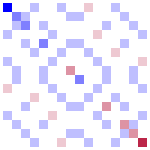
\includegraphics{imgs/3H.pdf}}\right), \hspace{5 mm} 
	\hat{U} = \left(\raisebox{-12mm}{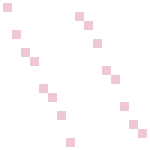
\includegraphics{imgs/3U.pdf}}\right), \hspace{5 mm} 
	\hat{U}\D\hat{H} \hat{U} = \left(\raisebox{-12mm}{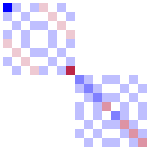
\includegraphics{imgs/3UHU.pdf}}\right). \hspace{5 mm} 
	\raisebox{-18mm}{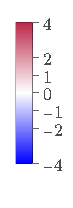
\includegraphics{imgs/3bl.pdf}}
\end{equation*}
where $\hat{U}$ represents reordering basis from
\begin{gather*}
	\ket{0000},\ket{0001},\ket{0010},\ket{0011},
	\ket{0100},\ket{0101},\ket{0110},\ket{0111}, \\
	\ket{1000},\ket{1001},\ket{1010},\ket{1011}, 
	\ket{1100},\ket{1101},\ket{1110},\ket{1111}
\end{gather*}
to 
\begin{gather*}
	\ket{0000},\ket{0011},\ket{0101},\ket{0110}, 
	\ket{1001},\ket{1010},\ket{1100},\ket{1111}, \\
	\ket{0001},\ket{0010},\ket{0100},\ket{0111},
	\ket{1000},\ket{1011},\ket{1101},\ket{1110}.
\end{gather*}


\begin{enumerate}[label=(\alph*)]
    \item To diagonalize $\hat{H}$ we could start from Fourier Transform
\begin{equation*}
	\hat{c}_k = \frac{1}{\sqrt{L}} \sum_j e^{i k j} \hat{c}_j,
	\hspace{10 mm} 
	\hat{c}_j = \frac{1}{\sqrt{L}} \sum_k e^{-i k j} \hat{c}_k.
\end{equation*}
Consider $L$ is even. If we want $\hat{c}_{L+1}= \hat{c}_1$ we have $H_1$ and
\begin{equation*}
	\mathcal K_{p=1} = \left\{
		k = \frac{\pi }{L}2n \ \big| \ n= - \tfrac{1}{2}L+1, \ldots, 0,\ldots,\tfrac{1}{2}L
	\right\},
\end{equation*}
otherwise $\hat{c}_{L+1} = - \hat{c}_1$ in $H_0$ and
\begin{equation*}
	\mathcal K_{p=0} = \left\{
		k =  \frac{ \pi }{L}(2n-1) \ \big| \  n= - \tfrac{1}{2}L+1, \ldots, 0,\ldots,\tfrac{1}{2}L
	\right\}.
\end{equation*}
And rewriting in terms of $\mathcal K_p$ hamiltonian we have
\begin{equation*}
	\hat{H}_{p} = -\sum_{k \in \mathcal K_p} (J \cos k + h) \left(
		\hat{c}\D_k \hat{c}_k - \hat{c}_{-k} \hat{c}\D_{-k}
	\right) - J \sum_{k \in \mathcal K_p} \left(e^{ik} \hat{c}_k\D \hat{c}_{-k}\D + \hc \right)
\end{equation*}

    \item It is useful to combine $k=0$ and $k=\pi$ for $p=1$
\begin{equation*}
	\hat{H}_{k=0,\pi} = - 2J (\hat{n}_0 - \hat{n}_\pi) + 2 h (\hat{n}_0 + \hat{n}_{\pi} - 2).
\end{equation*}
The remaining terms come into pairs $(k,-k)$, so we could go to the positive $k$:
\begin{align*}
	\mathcal K_1^+ &= \left\{
		k =  \frac{ \pi }{L}2n\ \big| \  n= 1,\ldots,\tfrac{1}{2}L-1
	\right\}, \\
	\mathcal K_0^+ &= \left\{
		k =  \frac{ \pi }{L}(2n-1) \ \big| \  n= 1,\ldots,\tfrac{1}{2}L
	\right\}.
\end{align*}
The $\hat{H}$ can be expressed as
\begin{equation*}
	\hat{H}_0 = \sum_{k \in \mathcal K_0^+} \hat{H}_k,
	\hspace{10 mm} 
	\hat{H}_1 = \hat{H}_{k=0,\pi} +  \sum_{k \in \mathcal K_1^+} \hat{H}_k,
\end{equation*}
with
\begin{equation*}
	\hat{H}_k = -2(J \cos k + h) \left(\hat{c}_k\D \hat{c}_k - \hat{c}_{-k} \hat{c}_{-k}\D\right) - 2 i J \sin k \left(
		\hat{c}_{k}\D \hat{c}_{-k}\D - \hat{c}_{-k} \hat{c}_{-k}
	\right).
\end{equation*}
Introducing $\hat{\Psi}\D_k = (\hat{c}_k\D,\ \hat{c}_{-k})$ we could simplify $\hat{H}_k$ to the
\begin{equation*}
	\hat{H} = \hat{\Psi}_k\D H_k \hat{\Psi}_k,
	\hspace{10 mm} 
	H_k = -2 J\begin{pmatrix}
	    -\tfrac{h}{J} + \cos k &  i \sin k \\
	    -  i \sin k & \tfrac{h}{J} - \cos k \\
	\end{pmatrix}.
\end{equation*}
Great, we have reduced the Hamiltonian to quadratic form and ready for the \textit{Bogolyubov transform}:
\begin{equation*}
	\hat{\Psi}_k = U \hat{\Phi}_k,
	\hspace{0.25cm} \Rightarrow \hspace{0.25cm}
	\hat{H}_k = \hat{\Phi}_k\D D_k \hat{\Phi}_k,
	\hspace{5 mm} 
	D_k = U\D H_k U = \begin{pmatrix}
	    \varepsilon_k & 0 \\
	    0 & -\varepsilon_k \\
	\end{pmatrix},
\end{equation*}
where $\hat{\Phi}_k\D \overset{\mathrm{def}}{=}   (\hat{\gamma}_k\D,\ \hat{\gamma}_{-k})$ -- our new operators. Diagonalizing $H_k$ we have
\begin{equation}
	U_k = \begin{pmatrix}
	    u_k & -\bar{v}_k \\
	    v_k & u_k \\
	\end{pmatrix} = 
	\frac{1}{\sqrt{\varepsilon_k(\varepsilon_k + z_k)}} \begin{pmatrix}
	    \varepsilon_k + z_k & i y_k \\
	    i y_k & \varepsilon_k + z_k \\
	\end{pmatrix},
	\hspace{5 mm} 
	\boxed{
	\varepsilon_k = 2 J \sqrt{\left(\cos k - \tfrac{h}{J}\right)^2 + \sin(k)^{2}}
	}
	\label{gap}
\end{equation}
where we introduced new parameters
\begin{equation*}
	u_k = \frac{\varepsilon_k + z_k}{\sqrt{\varepsilon_k (\varepsilon_k + z_k)}},
	\hspace{10 mm} 
	v_k = \frac{i y_k}{\sqrt{\varepsilon_k (\varepsilon_k + z_k)}},
	\hspace{10 mm} 
	\left.\begin{aligned}
    	z_k &= 2(h-J\cos k), \\
		y_k &= 2 J \sin k.
	\end{aligned}\right.
\end{equation*}
We could show that still
\begin{equation*}
	\{\hat{\gamma}_k, \hat{\gamma}_k\D\} = \{\bar{u}_k \hat{c}_k + \bar{v}_k \hat{c}\D_{-k},\ u_k \hat{c}_k\D + v_k \hat{c}_{-k}\} = |u_k|^2 + |v_k|^2 = 1,
\end{equation*}
so $\hat{\gamma}$ is a fermion. \red{Calculate commutators? But they are fermions!}


\end{enumerate}


	\item 
\begin{figure}[h]
    \centering
    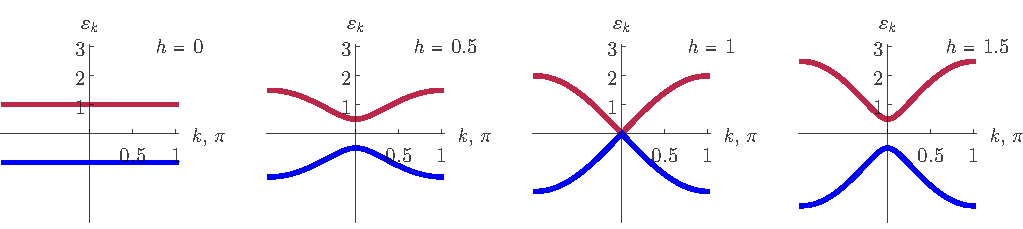
\includegraphics[width=0.9\textwidth]{imgs/3gap.pdf}
    \caption{TFIM dispersion with different magnetic fields $h$ with $J=1$}
    \label{fig:gap}
\end{figure}


\begin{enumerate}[label=(\alph*)]
    \item Ground state we could find in $\hat{H}_0$ such that $\hat{\gamma}_k \gs = 0 \ \forall k$. As in BCS theory we could start from some state (not orthogonal $\gs$), apply $\hat{\gamma}_k$ and normalize, coming to the
\begin{equation*}
	\gs = \frac{\prod_k \hat{\gamma}_{-k} \hat{\gamma}_k}{\left\|\prod_k \hat{\gamma}_{-k} \hat{\gamma}_k \ket{0}\right\|} \ket{0} = \prod_{k \in \mathcal K^+_0} \left(u_k + v_k \hat{c}_k\D \hat{c}\D_{-k}\right) \ket{0},
	\hspace{10 mm} 
	E_0 = - \sum_{k \in \mathcal K^+_0} \varepsilon_k,
\end{equation*}
with $\ket{0} \sim \ket{\downarrow\ldots\downarrow}$ -- vacuum for the original fermions $\hat{c}_k \ket{0} = 0 \ \forall k$. 
% \red{Add calculations of normalization.} 
% \red{Add proof that $p=1$ is not about ground state.} 
 If we want to continue exist in separated Hilbert space, than elementary excitation should save parity
\begin{equation*}
    \hat{\gamma}_{k_1}\D \hat{\gamma}_{k_2}\D \gs = \hat{c}_{k_1}\D \hat{c}_{k_2}\D \prod_{k \neq |k_1|,|k_2|}^{K^+_0} \left(\bar{u}_k - \bar{v}_k \hat{c}\D_k \hat{c}_{-k}\D \right) \ket{0}.
\end{equation*}
Going to the even amount of fermions we could apply even amount of $\hat{\gamma}_k$ to the $\gs$.
    \item Gap between minimal exitation and $\gs$ is $\varepsilon_{k=0}$,
% (we go from $-\varepsilon_k$ to the $\varepsilon_k$, that how 2-factor appear)
 and gap in $\varepsilon_k$ disappear at $h/J=1$ (fig. \ref{fig:gap}). Interesting to plot all $\hat{H}$ eigenvalues and see what is happening in the same values of $h$ (fig. \ref{fig:F}). 




\begin{figure}[h]
    \centering
    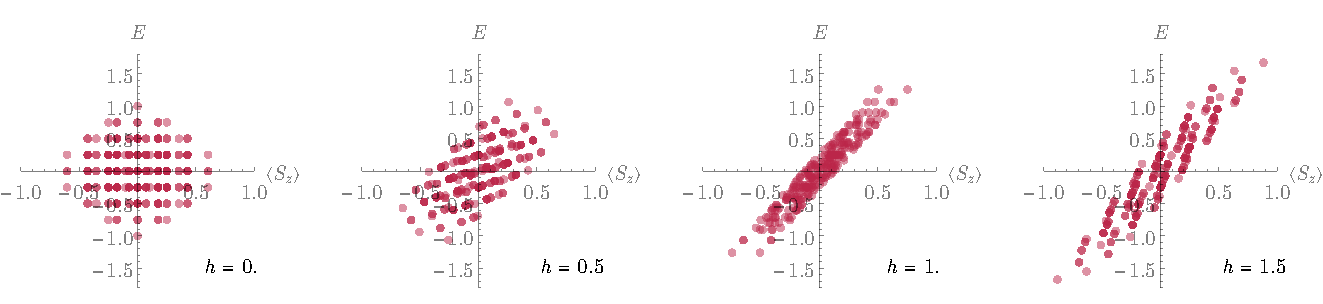
\includegraphics[width=0.9\textwidth]{imgs/3F.pdf}
    \caption{Eigenvalues of $\hat{H}$ as a function of $\langle S_z\rangle$}
    \label{fig:F}
\end{figure}

\end{enumerate}
 \newpage
	\item Consider $\xi$ as
\begin{equation*}
	f(r) = \left\langle \sigma_j^z \sigma_{j+r}\right\rangle \propto e^{- r /\xi},
\end{equation*}
so we could estimate it numerically (fig. \ref{fig:raf}). We have finite $L$ that strongly affects $\xi$ estimation, but definitely something interesting happens at $h=\sub{h}{c}=1$.

 We know that
\begin{equation*}
	\frac{1}{\sub{E}{gap} }  \propto \frac{1}{\varepsilon_{k=0}} \propto  \xi^{z} \propto (h - \sub{h}{c})^{-\nu z},
\end{equation*}
and from \eqref{gap} at $k=0$ we have $\sub{E}{gap} \propto h-1$, than $\sub{h}{c}=1$ and $\nu z = 1$.

\begin{figure}[h]
    \centering
    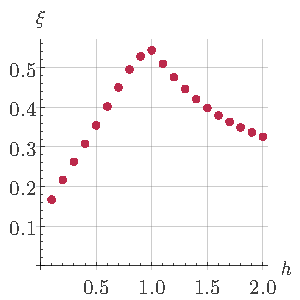
\includegraphics[width=0.25\textwidth]{imgs/3rad.pdf}
    \caption{Correlation radius $\xi$ as a function of external magnetic field $h$ at $L=20$, ground state}
    \label{fig:raf}
\end{figure}

\end{enumerate}





\newpage
\setcounter{section}{4}
% \section{Feynman Path Integral and Grassmannian Algebra}
\setcounter{subsection}{0}
\subsection{Feynman Path Integral of the Harmonic Oscillator}
Consider propagator as 
\begin{equation*}
	K \overset{\mathrm{def}}{=}  \bk{q_f}[e^{-i \hat{H} T}]{q_i},
\end{equation*}
that we could rewrite in terms of the Feinman's integral
\begin{equation*}
	K = \int e^{i S[q(t)]} \F q(t),
\end{equation*}
with in particular action for the harmonic oscillator
\begin{equation}
	S[q(t)] = \int_{0}^{T} \frac{m}{2} \left(
		\dot{q}^2 - \omega^2 q^2
	\right)
	\label{S}
\end{equation}
with boundary conditions $q(0) = q_i$ and $q(T) = q_f$. 

\begin{enumerate}[label=(\alph*)]
    
    \item Writing the path as $q(t) = q_c(t) = y(t)$, due to $\delta S[q_c(t)] = 0$ we could rewrite $S$ as 
\begin{equation*}
	S[q(t)] = \int_{0}^{T} \frac{m}{2}\left(
		(\dot{q}_c + \dot{y})^2 - \omega^2 (q_c + y)^2
	\right) \d t = S[q_c(t)] + S[y(t)] + \int_{0}^{T} m\left(
		\dot{q}_c \d y - \omega^2 q_c y \d t
	\right)  = S[q_c(t)] + S[y(t)].
\end{equation*}
It was used that Euler-Lagrange equation $\partial_x L - \frac{d }{d t} \partial_{\dot{x}} L = 0$ leads to classical equation of motion $\ddot{q}_c = - m \omega^2 q_c(t)$:
\begin{equation*}
	\int_{0}^{T}  m \dot{q}_c \d y = y(t) \dot{q}_c \bigg|_0^T - \int_{0}^{T} m y \ddot{q}_c \d t = \int_{0}^{T}  m \omega^2 y q_c \d t. 
\end{equation*}
Thus we could factorise $K$
\begin{equation*}
	K = e^{i S[q_c(t)]} F(T),
	\hspace{10 mm} 
	F(T) = \int e^{i S[y(t)]} \F y(t).
\end{equation*}

    \item Solving $\ddot{q}_c = - m \omega^2 q_c(t)$ with boundary conditions $q(0) = q_i$ and $q(T) = q_f$ we get
\begin{equation*}
	q_c(t) = A \cos (\omega t) + B \sin (t),
	\hspace{0.25cm} \Rightarrow \hspace{0.25cm}
	\left\{\begin{aligned}
	    q_i &= B \\
	    q_f &= A \sin(\omega T) + B \cos(\omega T)
	\end{aligned}\right.
	\hspace{0.25cm} \Rightarrow \hspace{0.25cm}
	A = \frac{q_f - q_i \cos(\omega T)}{\sin(\omega T)},
	\hspace{2.5 mm} 
	B = q_i,
\end{equation*}
and substituting into the action \eqref{S}
\begin{equation*}
	S[q_c(t)] = \frac{m \omega}{2 \sin(\omega T)} \left(
		(q_i^2 +q_f^2) \cos(\omega T) - 2 q_i q_f
	\right).
\end{equation*}
    \item The fluctuations can be expressed as a Fourier series
\begin{equation*}
	y(t) = \sum_{n=1}^{\infty} a_n \sin\left(
		\frac{n \pi t}{T}
	\right),
\end{equation*}
we go to the integration over $\prod_n a_n$. It is useful to calculate
\begin{equation*}
	\int_{0}^{T} \dot{y}^2 \d t = \frac{T}{2} \sum_{n=1}^{\infty} \left(\frac{\pi n}{T}\right)^2 a_n^2,
	\hspace{10 mm} 
	\int_{0}^{T} y^2 \d t = \frac{T}{2} \sum_{n=1}^{\infty} a_n^2.
\end{equation*}
So we could find $F$ as
\begin{equation*}
	F(T) \propto \int \exp\left(
		-\sum_{n=1}^{\infty} \alpha_n  a_n^2
	\right) \prod_n \d a_n = \prod_{n=1}^{\infty} \sqrt{\frac{\pi}{\alpha_n}},
	\hspace{10 mm} 
	\alpha_n = \frac{m}{2 i \hbar}\frac{T}{2} \left(\frac{\pi n}{T}\right)^2 \left(1 - \frac{\omega^2 T^2}{n^2 \pi^2}\right) .
\end{equation*}
Ignoring all factors without $\omega$, we have
\begin{equation*}
	F(T) = C \prod_{n=1}^{\infty} \left(1 -  \frac{\omega^2 T^2}{n^2 \pi^2}\right)^{-1/2} = C \sqrt{\frac{\omega T}{\sin (\omega T)}},
\end{equation*}
with some constant $C$ that could be find from the free particle case $\omega \to 0$
\begin{equation*}
	\lim_{\omega \to 0} F(T) = C = \sqrt{\frac{m}{2\pi i \hbar T}},
	\hspace{0.5cm} \Rightarrow \hspace{0.5cm}	
	F(T) = \sqrt{\frac{m \omega}{2\pi i \hbar \sin(\omega T)}}.
\end{equation*}
    \item[(d, e)] Now we could calculate the partition function $Z = \tr e^{- \beta \hat{H}}$ after a Wick rotation to imaginary times $T = - i \beta$
\begin{equation*}
	Z = \int \bk{x}[e^{- \beta \hat{H}}]{x} \d x = \int e^{i S[q_c(-i \beta)]}F(-i \beta) \d x \overset{(1)}{=}  \frac{1}{2 \sh\left(\tfrac{1}{2} \omega \beta\right)},
\end{equation*}
where in $\overset{(1)}{=}$ we calculated Gaussian integral 
\begin{equation*}
	\int \exp(- \alpha x^2) \d x = \sqrt{\frac{\pi}{\alpha}},
	\hspace{10 mm} 
	\alpha = \frac{ i m \omega \left(1 - \cos (\omega T)\right)}{\sin (\omega T)}.
\end{equation*}

\end{enumerate}





\subsection{Grassmannian Algebra}
\subsection{Grassmannian Algebra (I)}

We know, that for the Grassmann number $\eta$
\begin{equation*}
	\int \eta \d \eta = 1,
	\hspace{10 mm} 
	\int \d \eta = 0.
\end{equation*}

\begin{enumerate}
	\item Interesting to note, that for $f(\eta) = a + b \eta$ ($a,\, b \in \mathbb{C}$) we have
\begin{equation*}
	\{\eta,\, \partial_\eta\} f(\eta) = \{\eta,\, \textstyle \int d \eta\} f(\eta) = f(\eta).
\end{equation*}
Enough to calculate
\begin{equation*}
\textstyle
	\eta \int d \eta f(\eta) = b \eta,
	\hspace{5 mm} 
	\eta \partial_\eta f(\eta) = b \eta,
	\hspace{5 mm} 
	\int d \eta \eta  f(\eta) = a,
	\hspace{5 mm} 
	\partial_\eta \eta  f(\eta) = a.
\end{equation*}
	\item As a next step we calculate 
\begin{equation*}
	\exp\left(
		\sum_j c_j \eta_j
	\right) = 1 + \sum_j c_j \eta_j + 
	\sum_{j,k} c_j c_k \eta_j \eta_k = 
	 1 + \sum_j c_j \eta_j + 
	\sum_{j>k} c_j c_k (\eta_j \eta_k+\eta_k \eta_j) =  1 + \sum_j c_j \eta_j 
	,
\end{equation*}
with $c_j \in \mathbb{C}$. Actually it is the same as proof that $\sum_j c_j \eta_j $ is still Grassmann number by calculating anticommutative relations.
	\item Finally, we could find integral
\begin{equation*}
	\int d \bar{\eta} d \eta \ e^{- C \bar{\eta} \eta} = 
	\int d \bar{\eta} d \eta \left(
		1 - C \bar{\eta} \eta + \tfrac{C^2}{2} \bar{\eta}  \eta \bar{\eta} \eta + \ldots
	\right) = C \int d \bar{\eta} \left(
		\int d \eta\ \eta \bar{\eta}
	\right) = C,
\end{equation*}
with $C \in \mathbb{C}$. It was used that $\bar{\eta}  \eta \bar{\eta} \eta = - \bar{\eta}^2 \eta^2 = 0$.
\end{enumerate}




\newpage
\setcounter{section}{5}
% \section{Harmonic oscillator}
\setcounter{subsection}{0}
\subsection{Complex analysis}
Consider Gaussian integral 
\begin{equation*}
	I_1 = \int_{-\infty}^{\infty} e^{-i a x^2} \d x,
\end{equation*}
with $\alpha \in \mathbb{R}^+$. We could use that
\begin{equation*}
	I_2 = \int_{-\infty}^{\infty} e^{-b x^2} \d x = \sqrt{\frac{\pi}{a}}.
\end{equation*}
Define  $\mathcal C_1 = \{z=e^{i \frac{\pi}{4}x} \colon x \in \mathbb{R}\}$,
$\mathcal C_2 = \{z=x \colon x \in \mathbb{R}\}$ and ${\mathcal C}_R^\pm = \{z = \pm R e^{i \varphi} \colon \varphi \in [0, \pi/4]\}$. Applying Cauchy integral theorem for holomorphic functions to the $\mathcal C = \mathcal C_1 \cup \mathcal C_2 \cup {\mathcal C}_R^+ \cup {\mathcal C}_R^-$ we have 
\begin{equation*}
	-I[\mathcal C_1]+I[\mathcal C_2]+I[{\mathcal C}_R^+]+I[{\mathcal C}_R^-] = 0,
\end{equation*}
with $I[\mathcal C_1] e^{-i \frac{\pi}{4}} = I_1 $, $I[\mathcal C_2] = I_2$.

The $I[{\mathcal C}_R^\pm]$ could be estimated as
\begin{equation*}
	|I[{\mathcal C}_{R \to \infty}^\pm] | \leq \lim_{R \to \infty} \int_{0}^{\pi/2} e^{-a R^2 \varphi} r \d \varphi = \lim_{R \to \infty} \frac{1}{aR}\left(
		1 - e^{- \frac{1}{2} a \pi r^2}
	\right) = 0,
\end{equation*}
thus we have
\begin{equation*}
	I_1 = I[\mathcal C_1] e^{-i \frac{\pi}{4}} =  I[\mathcal C_2] e^{-i \frac{\pi}{4}} = e^{-i \frac{\pi}{4}} \sqrt{\frac{\pi}{a}},
\end{equation*}
that could be generalized as
\begin{equation*}
	\int_{-\infty}^{\infty} e^{\pm i a x^2} \d x = e^{\pm i \frac{\pi}{4}} \sqrt{\frac{\pi}{a}}.
\end{equation*}



\subsection{Effective action of coupled harmonic oscillators}
We could derive the low-energy effective action for a system of two
coupled harmonic oscillators, formally described by the classical partition function
\begin{equation*}
	Z = \int Dx DX \, \exp\left(
		i \int dt\ L(x, X, \dot{x}, \dot{X}) 
	\right),
\end{equation*}
with
\begin{equation*}
	L = \frac{1}{2} m \dot{x}^2 - \frac{1}{2} m \omega^2 x^2 + \frac{1}{2} M \dot{X}^2 - \frac{1}{2} M \Omega^2 X^2 - g X x.
\end{equation*}
It could be expanded as
\begin{equation*}
	Z = \int Dx \ e^{i S_0 + i\sub{S}{int}},
	\hspace{5 mm} 
	e^{ i\sub{S}{int}} = \int D X \ \exp\left(
		i \int \d t \left[
			\tfrac{1}{2} M \dot{X}^2 - \tfrac{1}{2} M \Omega^2 X^2 - g X x
		\right]
	\right).
\end{equation*}
Integrating by parts we have Gaussian integral that coul be calculated directly
\begin{equation*}
	e^{ i\sub{S}{int}} = \int D X \ \exp\left(
		i \int \d t \left[
			\tfrac{1}{2} M X(\partial_t^2+ \Omega^2)X - g X x
		\right]
	\right) = \mathcal N \exp\left(
		i \int dt \frac{g^2}{2M} x \left(\partial_t^2 + \Omega^2\right)^{-1} x
	\right)
\end{equation*}
with $\mathcal N$ as some irrelevant normalizing factor. That leads to some $\sub{L}{eff}$
\begin{equation*}
	\sub{L}{eff} = \tfrac{1}{2} m \ddot{x}^2 - \frac{1}{2} m x^2 \sub{\omega}{eff}^2,
	\hspace{10 mm} 
	\sub{\omega}{eff} =  \omega \sqrt{1 - \alpha^2 \frac{m}{M} \left(\frac{\omega}{\Omega}\right)^2},
\end{equation*}
with $g = \alpha m \omega^2$ and, apparently, $\sub{m}{eff} = m$.






\newpage
\setcounter{section}{6}
% \section{Green’s functions and Heisenberg model}
\setcounter{subsection}{0}
\subsection{Thermal Green’s functions}
The thermal Green's function is defined as 
\begin{equation*}
	G_{ij}(\tau) = - \langle \text{T}_\tau\ \psi_i(\tau) \psi_j\D (0) \rangle
\end{equation*}
The path integral formulation of the Green's function of non-interacting particles is
\begin{equation}
	G_{ij}(\tau) = - \frac{1}{Z} \int D(\bar{\psi}, \psi) \psi_i(\tau) \bar{\psi}_j(0) e^{-S[\bar{\psi}, \psi]},
	\hspace{10 mm} 
	S = \sum_j \int_0^\beta d\tau\, \bar{\psi}_j (\partial_\tau + \varepsilon_j - \mu) \psi_j = \sum_j 
	s[\bar{\psi}_j, \psi_j].
	\label{PIGF}
\end{equation}

\textbf{1. Time ordering}. 
The path integral automatically takes care of the time ordering:
\begin{equation*}
	G_{ij}(\tau>0) = -\langle \psi_i(\tau) \psi_j\D(0)\rangle = \tr\left(
		e^{-(\beta-\tau) H}  \psi_i e^{-H \tau} \psi_j\D
	\right),
\end{equation*}
and than we could repeat the construction of the path integral and get \eqref{PIGF}. In other case
\begin{align*}
	G_{ij}(\tau<0) &= \zeta \langle \psi_j\D(0) \psi_i(\tau)\rangle = 
		\tr\left(
		 \psi_j\D  e^{-(-\tau)H} \psi_i e^{-(\beta+\tau)H}
	\right)
	\\
	&= - \frac{\zeta}{Z} \int D(\bar{\psi}, \psi) \bar{\psi}_j(0) \psi_i(\tau)  e^{-S(\bar{\psi}, \psi)} = - \frac{\zeta^2 }{Z} \int D(\bar{\psi}, \psi) \psi_i(\tau) \bar{\psi}_j(0) e^{-S(\bar{\psi}, \psi)},
\end{align*}
thus we come to the same \eqref{PIGF}.


\textbf{2. Green's function as Matsubara sum}. After the Fourier transform (unitary)
\begin{equation}
	\psi_j(\tau) = \frac{1}{\sqrt{\beta}} \sum_n e^{- i \omega_n \tau} \psi_{jn},
	\hspace{10 mm} 
	\omega_n = \frac{\pi}{\beta}\left\{\begin{aligned}
	    &2n+1, &\text{fermions}, \\
	    &2n, &\text{bosons}, \\
	\end{aligned}\right.
	\label{omegadef}
\end{equation}
we get 
\begin{equation}
	G_{ij}(\tau) = - \frac{1}{Z} \frac{1}{\beta} \sum_{n,m} \int D(\bar{\psi}, \psi) 
	e^{-i \omega_n \tau} \psi_{in} 
	\bar{\psi}_{jm} e^{-S[\bar{\psi}, \psi]},
	\hspace{10 mm} 
	S = \sum_{j,n} \bar{\psi}_{jn} (- i \omega_n + \varepsilon_j - \mu) \psi_{jn}.
	\label{ftgf}
\end{equation}
We could simplify calculations noticing that due to the sign symetry of the action
\begin{equation*}
	\int d(\bar{\psi}_j, \psi_j) \psi_{j n} e^{-s[\bar{\psi}_{jn}, {\psi}_{jn}]} = 0,
	\hspace{0.5cm} \Rightarrow \hspace{0.5cm}
	G_{i,j \neq i} (\tau) = 0.
\end{equation*}
To the next simplification in $G_{jj}(\tau)$ we could factor
\begin{equation*}
	I_{nm}^j = \int d(\bar{\psi}_{jn},{\psi}_{jn})\, d(\bar{\psi}_{jm},{\psi}_{jm})\, \psi_{jn} \bar{\psi}_{jm} e^{-s[\bar{\psi}_{jn}, \psi_{jn}]} e^{-s[\bar{\psi}_{jm},{\psi}_{jm}]} \propto \delta_{nm}
\end{equation*}
again due to the symmetry. It is useful to rewrite $I_{nn}^j$ as
\begin{equation*}
	I_{nn}^j = 
	 	\red{\int d(\bar{\psi}_{jn}, \psi_{jn})  \psi_{jn} \bar{\psi}_{jn} e^{-s[\bar{\psi}_{jn}, \psi_{jn}]}}
	 	\blue{\int d(\bar{\psi}_{jn}, \psi_{jn}) e^{-s[\bar{\psi}_{jn}, \psi_{jn}]}}
	 = \red{\frac{1}{-i \omega_n + \varepsilon_j - \mu}}
	 \blue{\int d(\bar{\psi}_{jn}, \psi_{jn}) e^{-s[\bar{\psi}_{jn}, \psi_{jn}]}}.
\end{equation*}
It remains to note that <<blue>>-term helps us to factorize partition function in the \eqref{ftgf}
\begin{equation*}
Z = \bigg(\prod_{k \neq j} 
			\int d(\bar{\psi}_{k},{\psi}_{k})  e^{- \sum_{k \neq j} s[\bar{\psi}_{k}, \psi_{k}]}\bigg)
			\cdot
	\bigg(\prod_{m\neq n} 
			\int d(\bar{\psi}_{jm},{\psi}_{jm})  e^{-s[\bar{\psi}_{jm}, \psi_{jm}]}\bigg)
		\cdot
	\left(\blue{\int d(\bar{\psi}_{jn}, \psi_{jn}) e^{-s[\bar{\psi}_{jn}, \psi_{jn}]}} \right)
\end{equation*}
Finally $G_{ij}(\tau)$ could be expressed as
\begin{equation}
	G_{ij}(\tau) = \frac{\delta_{ij}}{\beta} \sum_n e^{- i \omega_n \tau} G_0(j, i \omega_n),
	\hspace{10 mm} 
	G_0(j, i \omega_n) \overset{\mathrm{def}}{=}  \frac{1}{i \omega_n - \varepsilon_j + \mu}
	.
	\label{gfdef}
\end{equation}

% \textbf{Calculating the Matsubara sum}. 
Substituting $\omega_n$ from \eqref{omegadef} as usual $G_{ij}(\tau)$ could be rewritten as
 % Following Jordan's lemma we need consider two cases of $\sign(\tau)$:
\begin{align}
	G_{jj}(\tau > 0)  
	&=
	-\zeta \oint \frac{dz}{2\pi i} \frac{e^{-z \tau}}{z-\xi_j} \nBF(-z), \\
	G_{jj}(\tau < 0)  
	&=
	-\zeta \oint \frac{dz}{2\pi i} \frac{e^{z \tau}}{-z+\xi_j} \nBF(z),
\end{align}
with $\xi_j \overset{\mathrm{def}}{=} \varepsilon_j-\mu$ and $\nBF(z) = (e^{\beta z} - \zeta)^{-1}$. Sign of $z$ was chosen to provide convergence. Summing over the outer pole we get 
\begin{align*}
	G_{jj}(\tau > 0) &= \zeta \nBF(-\xi_j) e^{- \xi_j \tau}, \\
	G_{jj}(\tau < 0) &= -\zeta \nBF(\xi_j) e^{- \xi_j \tau}.
\end{align*}
Combining all this happiness into one expression
\begin{equation}
	\boxed{
	G_{ij}(\tau) = -\delta_{ij} \left(
		\theta(\tau) + \zeta \nBF(\xi_j)
	\right) e^{-\xi_j \tau}
	}.
	\label{res}
\end{equation}
In general, it is quite logical to obtain the theta function due to T-ordering, since $\hat{a}\hat{a}\D = 1 + \zeta \hat{a}\D \hat{a} $.


% Important to notice, that 
% \begin{equation*}
% 	G_{jj}(\tau)^{-1} G_{jj}(\tau) = - ( \partial_\tau + \xi_j)\left(
% 		\theta(\tau) + \zeta \nBF(\xi_j)
% 	\right) e^{-\xi_j \tau} = - e^{-\xi_j \tau} \partial_\tau \theta(\tau) = - \delta (\tau),
% \end{equation*}
% with $G_{jj}(\tau)^{-1} = \partial_\tau + \xi_j$. 
% \textcolor{grey}{Although it confuses me a little that this is done as if for any kind of function instead $\nBF$.}

\textbf{3. The occupation number}. The occupation number in a single particle state  $j$ is in general given by
\begin{align*}
	n_j &= \langle \psi_j\D(0) \psi_j(0)\rangle 
	= \zeta \lim_{\tau \to 0^-} \langle \text{T}_{\tau} \psi_i(\tau) \psi_j\D \rangle = - \zeta \lim_{\tau \to 0^-} G_{jj}(\tau), \\
	&\textcolor{grey}{= \zeta \lim_{\tau \to 0^+} \langle \text{T}_{\tau} \psi_i(\tau) \psi_j\D-1\rangle =  \zeta \lim_{\tau \to 0^+} (-G_{jj}(\tau)-1 )
	% \ \text{or something like this.}
	} 
\end{align*}
Expanding \eqref{res} we get
\begin{equation*}
	n_j =  - \zeta \lim_{\tau \to 0^-} G_{jj}(\tau) = \zeta^2 \nBF(\xi_j) \lim_{\tau \to 0^-} e^{-\xi_j \tau} = \nBF(\xi_j).
\end{equation*}


\textbf{4. The generating functional}. The generating functional for correlation functions is defined as
\begin{equation*}
	\Z[\bar{J}, J] = \int D\left(\bar{\psi}, \psi\right) \, \exp\bigg(
		- S[\bar{\psi}, \psi] - \sum_j \int_{0}^{\beta} d \tau\left(
			\bar{J}_j \psi_j + \bar{\psi}_j J_j
		\right)
	\bigg).
\end{equation*}
These can be obtained as functional
derivatives of $\Z[\bar{J},J]$, where the source fields are set to zero after the evaluation:
\begin{equation*}
	\langle 
		\text{T}_\tau \psi_{in} \psi_{jm}
	\rangle = \frac{\zeta}{\Z[0,0]} \frac{\delta^{2} \Z[\bar{J},J]}{\delta \bar{J}_{in} \delta J_{jm}} \bigg|_{J, \bar{J}=0}.
\end{equation*}
It remains to calculate
\begin{align*}
	\Z[\bar{J},J] &= \int D(\bar{\psi}, \psi) \ \exp\bigg(
		- \sum_{j, n} \bar{\psi}_{jn} \left(-G_0^{-1}(j, i \omega_n)\right) \psi_{jn} + \sum_{j,n} \bigg(
			\bar{J}_{jn} \psi_{jn} + \bar{\psi}_{jn} J_{jn}
		\bigg)
	\bigg) 
	\\ &=  \Z[0,0] \exp\bigg(
		- \sum_{j,n} \bar{J}_{jn} G_0(j, i \omega_n) J_{jn}
	\bigg).
\end{align*}
Thus for the Green's function $G_{ij}(i \omega_n)$ in Matsubara space 
\begin{equation*}
	G_{ij}(i \omega_n) = -\langle 
		\text{T}_\tau \psi_{in} \psi_{jm}
	\rangle = -\zeta \frac{\delta^2}{\delta \bar{J}_{in} \delta J_{jm}} \exp\bigg(
		- \sum_{j,n} \bar{J}_{jn} G_0(j, i \omega_n) J_{jn}
	\bigg) \bigg|_{\bar{J}=J=0} = \delta_{ij} \delta_{nm} G_0(j, i \omega_n),
\end{equation*}
corresponding to \eqref{gfdef}.


% In general
% \begin{align*}
% 	\Z_A[\bar{J}, J] = \int D(\bar{\psi}, \psi) \exp\left(
% 		- \int_{0}^{\beta} \d \tau \sum_{j}\left(\bar{\psi}_{j} A^{-1} \psi_{j} - \bar{J}_j \psi_j - \bar{\psi}_j J_j\right) 
% 	\right) = \Z[0,0] e^{- \bar{J} A J}.
% \end{align*}
% In our case $A=G_{ij}(\tau)$


% \begin{align*}
% 	\Z[\bar{J}, J] = \int D(\bar{\psi}, \psi) \exp\left(
% 		- \int_{0}^{\beta} \d \tau \sum_{jn}\left(\bar{\psi}_{jn} (-i \omega_n + \varepsilon_j - \mu)\psi_{jn} - \bar{J}_j \psi_j - \bar{\psi}_j J_j\right) 
% 	\right) 
	% &= Z[0,0] \exp\left(
	% 	-\int_{0}^{\beta} d \tau \d \tau' \sum_{n,m} 
	% 	\bar{J}_n(\tau) 
	% \right)
% \end{align*}

\subsection{Nambu-Goldstone Modes in the Heisenberg Ferromagnet}
We consider an isotropic Heisenberg ferromagnet with spin 1/2-particles fixed to the sites of a lattice:
\begin{equation*}
	\hat{H} = - \frac{1}{2} \sum_{ij} J_{ij} \hat{\vc{S}}_i \cdot \hat{\vc{S}}_j,
\end{equation*}
with $J_{ij} > 0$. Let us label the ground states by their orientation in space:
\begin{equation*}
	\ket{0_{\vc{n}}} = \bigotimes_{i=1}^N \ket{i, \vc{n}},
\end{equation*}
with the single site states satisfying $\vc{n} \cdot \hat{\vc{S}}_j \ket{j, \vc{n}} = - \frac{1}{2} \ket{j, \vc{n}}$.

\textbf{1. Orthogonal states}. In spherical coordinates the single site state could be found from
\begin{equation*}
	\vc{n} \cdot \hat{\vc{S}} = \frac{1}{2} \left(
	\begin{array}{cc}
	 \cos (\theta ) & e^{-i \varphi } \sin (\theta ) \\
	 e^{i \varphi } \sin (\theta ) & -\cos (\theta ) \\
	\end{array}
	\right),
\end{equation*}
with eigenstate
\begin{equation*}
	\ket{0_{\vc{n}}} = \frac{\cos(\theta)-1}{\sqrt{2-2 \cos (\theta )}}\ket{\uparrow} + \frac{e^{i \varphi} \sin \theta}{\sqrt{2-2 \cos (\theta )}}\ket{\downarrow}.
\end{equation*}
We need projection to the $\ket{\downarrow}$, that could be simplified to the
\begin{equation*}
	|\bk{\downarrow}{0_{\vc{n}}}| = \bigg|\frac{2 \sin\left(\tfrac{1}{2}\theta\right)\cos\left(\tfrac{1}{2}\theta\right)}{2 \sin(\tfrac{1}{2}\theta)}\bigg| = |\cos(\tfrac{1}{2}\theta_{\downarrow \vc{n}})|
\end{equation*}
In the thermodynamic limit $N \to \infty$ 
\begin{equation*}
	| \bk{0_{ \vc{n}_1}}{0_{ \vc{n}_2}}| = \lim_{N \to \infty} |\cos(\tfrac{1}{2}\theta_{ \vc{n}_1 \vc{n}_1})|^N = 0.
\end{equation*}

\textbf{2. Hamiltonian}. We could substitute
\begin{equation*}
	\hat{S}^x = \tfrac{1}{2}\left(\hat{S}^+ + \hat{S}^-\right),
	\hspace{5 mm} 
	\hat{S}^y = \tfrac{1}{2i}\left(\hat{S}^+ - \hat{S}^-\right),
	\hspace{5 mm} 
	\hat{S}^z = \hat{S}^+ \hat{S}^- - \tfrac{1}{2},
\end{equation*}
that leads to terms as
\begin{align*}
	\hat{S}^x_i \hat{S}^x_j &= \tfrac{1}{4}\left(
		\red{\hat{S}^{+}_{i} \hat{S}^{+}_{j}} + \hat{S}^{+}_{i} \hat{S}^{-}_{j}  + \hat{S}^{-}_{i} \hat{S}^{+}_{j} + \red{\hat{S}^{-}_{i} \hat{S}^{-}_{j} }
	\right) \\
	\hat{S}^{y}_{i} \hat{S}^{y}_{j} &= \tfrac{-1}{4}\left(
		\red{\hat{S}^{+}_{i} \hat{S}^{+}_{j}} - \hat{S}^{+}_{i} \hat{S}^{-}_{j} - \hat{S}^{-}_{i} \hat{S}^{+}_{j} + 
		\red{\hat{S}^{-}_{i} \hat{S}^{-}_{j} }
	\right) \\
	\hat{S}^{z}_{i} \hat{S}^{z}_{j} &= \hat{S}^{+}_{i} \hat{S}^{-}_{i} \hat{S}^{+}_{j} \hat{S}^{-}_{j} - \tfrac{1}{2} \hat{S}^{+}_{i} \hat{S}^{-}_{i} - \tfrac{1}{2} \hat{S}^{+}_{j} \hat{S}^{-}_{j} + \tfrac{1}{4},
\end{align*}
so the Hamiltonian 
\begin{equation*}
	\hat{H} = -\frac{1}{2} \sum_{ij} J_{ij} \left(
		-\tfrac{1}{2} \left(\hat{S}^{+}_{i} - \hat{S}^{+}_{J} \right) \left(\hat{S}^{-}_{i} - \hat{S}^{-}_{j} \right) + \hat{S}^{+}_{i} \hat{S}^{-}_{i} \hat{S}^{+}_{j} \hat{S}^{-}_{j} + \tfrac{1}{4}
	\right).
\end{equation*}

\textbf{3. One-particle Hamiltonian}. We can reduce the Hilbert space to the one-particle states $\ket{j} = \hat{S}^{+}_{j} \ket{0_{\uparrow}}$. Neglecting constant terms, reduced Hamiltonian $\hat{H}'$
\begin{equation*}
 H'|i\rangle = -\frac{1}{2} \sum_{k j} J_{k j} \left(  - \frac{1}{2} \left( \delta_{ k i } | k \rangle - \delta_{j i} | k\rangle - \delta_{k i} |  j\rangle +  \delta_{j i }| j \rangle     \right) + \delta_{j i} \delta_{k j} | k \rangle   \right)   = \frac{1}{2} \sum_j J_{i j}(|i\rangle-|j\rangle)
\end{equation*}
with  matrix elements
\begin{equation*}
	\bk{i}[\hat{H}]{i} = \frac{1}{2} \sum_j J_{ij},
	\hspace{5 mm} 
	\bk{j}[\hat{H}]{i} = -\frac{1}{2} \sum_j J_{ij}.
\end{equation*}
Assuming $J_{ij} = J(|\vc{x}_i - \vc{x}_j|)$ consider the plane wave state $\ket{k} = \sum_j e^{i \vc{k} \vc{x}_j} \ket{j}$:
\begin{align*}
	\hat{H}' \ket{k} = \sum_i e^{i \vc{k} \vc{x}_i} \tfrac{1}{2} \sum_{j} J_{ij} \left(\ket{i} - \ket{j}\right).
\end{align*}
To simplify calculations consider
\begin{align*}
	\bk{m}[\hat{H}']{k} = \sum_i e^{i \vc{k} \vc{x}_i} \tfrac{1}{2} \sum_{j} J_{ij} \left(\delta_{mi} - \delta_{mj}\right) = e^{i \vc{k} \vc{x}_m} \tfrac{1}{2} \sum_j J_{mj} - \sum_j e^{i \vc{k} \vc{x}_j} \tfrac{1}{2} J_{jm}=  \tfrac{1}{2} \sum_j J_{jm} \left(1 - e^{i \vc{k}(\vc{x}_j - \vc{x}_m)}\right) e^{i \vc{k} \vc{x}_m}.
\end{align*}
We could sum over $\vc{x}_n = \vc{x}_j - \vc{x}_m$ and notice that $J_{jm} = J(|\vc{x}_j - \vc{x}_m|) = J(|\vc{x}_n|)$
\begin{equation*}
	\bk{m}[\hat{H}']{k}  = \frac{1}{2} \bigg(
		\sum_n J_{n0} \left(1-e^{i \vc{k} \vc{x}_n}\right)
	\bigg) e^{i \vc{k} \vc{x}_m} = E_{\vc{k}} \bk{m}{k},
\end{equation*}
thus we have proven that $\ket{k}$ is eigenstate with energy $E_{\vc{k}}$
\begin{equation*}
	E_{\vc{k}} = \frac{J_0 - J_k}{2},
	\hspace{10 mm} 
	J_k = \sum_j J(|x_j|) e^{-i \vc{k} \vc{x}_j}.
\end{equation*}
For a constant nearest neighbour interaction on a square lattice $E_{\vc{k}}$ could be calculated explicitly:
\begin{equation*}
	J_k = \sum_{\vc{x}_j = \pm \vc{e}_{x,y}} J(|\vc{x}_j|) e^{- i \vc{k} \vc{x}_j} = 2 J\left(
		\cos k_x + \cos k_y
	\right),
\end{equation*}
and energy
\begin{equation*}
	E_k = J\left(2 - \cos k_x - \cos k_y \right) \overset{k \to 0}{\approx} \frac{J}{2}\left(k_x^2 + k_y^2\right).
\end{equation*}




\newpage
\setcounter{section}{7}
\setcounter{subsection}{0}
% \section{Wick's theorem and Bogoliubov}
\subsection{Operator Identity for Gaussian Theories}
\textbf{General case.} To form some intuition, let's start with the proof
\begin{equation}
	\langle e^{\sum_j b_j x_j}\rangle = e^{\frac{1}{2}\sum_{i,j} b_i \langle x_i x_j \rangle b_j},
	\label{gen}
\end{equation}
with averaging defined as
\begin{equation*}
	\langle f\rangle = \frac{1}{Z} \int D(\vc{x}) f(\vc{x}) e^{- \frac{1}{2} \vc{x}\T G^{-1} \vc{x}}, \hspace{10 mm} 
	D(x) = \prod_n d x_n,
\end{equation*}
with $Z = \sqrt{\det(2\pi G)}$ so that $\langle 1\rangle = 1$. Both parts of the \eqref{gen} could be calculated directly:
\begin{equation*}
	\langle e^{\sum_j b_j x_j}\rangle = 
	\frac{1}{Z} \int D(x) e^{-\frac{1}{2} \vc{x}\T G^{-1} \vc{x} + \vc{b} \vc{x}} = \frac{1}{Z} \int D(\vc{x}) e^{- \frac{1}{2}(\vc{x}-G \vc{b})\T G^{-1} (\vc{x}-G \vc{b})}e^{\frac{1}{2} \vc{b}\T G \vc{b}},
\end{equation*}
and with $\vc{x}' = \vc{x} - G \bar{b}$ and $D(\vc{x}') = D(\vc{x})$ 
\begin{equation*}
	\langle e^{\vc{b} \vc{x}}\rangle = \frac{1}{Z} \int D(\vc{x}') e^{- \frac{1}{2} \vc{x}'{}\T G^{-1} \vc{x}'} e^{\frac{1}{2} \vc{b}\T G \vc{b}} = e^{\frac{1}{2} \vc{b}\T G \vc{b}} = e^{\frac{1}{2} \sum_{i,j} b_i \langle x_i x_j\rangle b_j},
\end{equation*}
with proved in the previous homework fact that $\langle x_i x_j\rangle = G_{ij}$.

\textbf{Special case}. We want to prove the operator identity
\begin{equation}
	\langle e^{i(\varphi(r)-\varphi(0))}\rangle = e^{- \frac{1}{2} \langle (\varphi(r)-\varphi(0))^2\rangle}.
	\label{base12}
\end{equation}
With $b(r') = i \delta(r'-r) - i \delta(r')$:
\begin{equation*}
	\sum_j b_j \varphi_j = \int b(r') \varphi(r') \d r' = i (\varphi(r)-\varphi(0)),
\end{equation*}
and for other part $\sum_{i,j} b_i \langle x_i x_j\rangle b_j = \langle  \sum_{i,j} b_i  x_i x_j b_j\rangle$, so
\begin{equation*}
	\sum_{i,j} b_i  x_i x_j b_j = \int
	b(r') \varphi(r') \varphi(r'') b(r'')
	\d r' \d r'' = \bigg(
		\int b(r') \varphi(r') \d r'
	\bigg)^2 = - (\varphi(r)-\varphi(0))^2,
\end{equation*}
thus we proved \eqref{base12} using \eqref{gen}.


\textbf{Wick's theorem}. Note that from \eqref{gen} are convenient to obtain Wick’s theorem \red{maybe}. Expanding \eqref{gen} in the Taylor series we have from the LHS
\begin{equation*}
	\langle e^{\sum_j b_j x_j}\rangle = 1 + \frac{1}{2!} \sum_{i,j} b_i b_j \langle x_i x_j\rangle + \frac{1}{4!}  \sum_{i,j,k,l} b_i b_j b_k b_l \langle x_i x_j x_k x_l\rangle + \ldots
\end{equation*}
and from the RHS 
\begin{equation*}
	e^{\frac{1}{2}\sum_{i,j} b_i \langle x_i x_j \rangle b_j} 1 + \frac{1}{2} \sum_{i,j} b_i b_j \langle x_i x_j\rangle + \sum_{i,j,k,l} b_i b_j b_k b_l \langle x_i x_j\rangle \langle x_k x_l\rangle + \ldots,
\end{equation*}
so collecting terms with proper $B^4$ we get
\begin{equation*}
	\langle x_i x_j x_k x_l\rangle = \langle x_i x_j\rangle \langle x_i x_k\rangle \langle x_j x_l\rangle + \langle x_i x_l\rangle \langle x_j x_k\rangle.
\end{equation*}
This result is known as Wick's theorem.
\newpage
\subsection{Bogoliubov theory}

\textbf{1. Hamiltonian}. 
Consider a microscopic Hamiltonian for bosons with weak contact interactions:
\begin{equation}
	\hat{H} - \mu \hat{N} = \sum_p (\varepsilon_p - \mu) \hat{a}_p\D \hat{a}_p + \frac{\varphi}{2V} \sum_{p, p', q} \hat{a}\D_{p+q} \hat{a}\D_{p'-q} \hat{a}_{p'} \hat{a}_p,
	\label{BECbase}
\end{equation}
where $\varepsilon_p = p^2 / 2m$ and second term as $\hat{V}$.  For $\varphi = 0$ the groundstate in a grandcanonical description is a coherent
state of bosons in the zero-momentum state, i.e. all particles are Bose condensed. 

Finite interactions lead to scattering of bosons from the condensate into finite momentum modes
and hence a depletion of the condensate fraction. However, if the interactions are weak,
one can still assume that the $p = 0$ mode is macroscopically occupied, $\langle a_0\D a_0\rangle \gg 1$. As $[a_0, a_0\D]=1$, one can neglect it for a macroscopically occupied $p = 0$ mode and replace $a_0,\ a_0\D$ by their expectation value $\sqrt{N_0}$, the number of bosons in the condensate. Thus our small parameter is $(N-N_0)/N_0$. One can therefore approximate all other modes to be small $a_p \ll \sqrt{N_0}$ and  therefore neglect all terms in the interaction part of above Hamiltonian which contain more than two creation/annihilation operators with $p \neq 0$. 


\begin{figure}[h]
    \centering
% a
\begin{tikzpicture}
	\begin{feynman}[small]
	\vertex (i1);
	\vertex [below right=of i1] (a);
	\vertex [below left=of a] (i2);
	\vertex [right=of a] (b);
	\vertex [above right=of b] (f1);
	\vertex [below right=of b] (f2);
	\diagram* {
	(i1) -- [scalar] (a) -- [scalar] (i2),
	(f1) -- [scalar] (b) -- [scalar] (f2),
	(a) -- [boson] (b),
	};
	\end{feynman}
\end{tikzpicture}
    \caption{Interaction of condensate particles}
    \label{fig:BCa}
\end{figure}


The leading term of the expansion involves interactions solely between the stationary particles (particles of the condensate) as in fig. \ref{fig:BCa} (the dashed line corresponds to condensed particles)
\begin{equation*}
	\hat{V}_0 = \frac{\varphi}{2V} \hat{a}\D_0 \hat{a}\D_0 \hat{a}_0 \hat{a}_0.
\end{equation*}
There are no terms that contain only one creation or annihilation operator for non-condensate particles due to the conservation of momentum.


\begin{figure}[h]
    \centering
% б
\begin{tikzpicture}
	\begin{feynman}[small]
	\vertex (i1);
	\vertex [below right=of i1] (a);
	\vertex [below left=of a] (i2);
	\vertex [right=of a] (b);
	\vertex [above right=of b] (f1);
	\vertex [below right=of b] (f2);
	\diagram* {
	(i1) -- [scalar] (a) -- [fermion, edge label=\(p\)] (i2),
	(f1) -- [fermion, edge label'=\(p\)] (b) -- [scalar] (f2),
	(a) -- [boson] (b),
	};
	\end{feynman}
\end{tikzpicture}
\hspace{5 mm} 
% в
\begin{tikzpicture}
	\begin{feynman}[small]
	\vertex (i1);
	\vertex [below right=of i1] (a);
	\vertex [below left=of a] (i2);
	\vertex [right=of a] (b);
	\vertex [above right=of b] (f1);
	\vertex [below right=of b] (f2);
	\diagram* {
	(f1) -- [scalar] (b) -- [fermion, edge label'=\(p\)] (f2),
	(i1) -- [fermion, edge label=\(p\)] (a) -- [scalar] (i2),
	(a) -- [boson] (b),
	};
	\end{feynman}
\end{tikzpicture}
\hspace{5 mm} 
% г
\begin{tikzpicture}
	\begin{feynman}[small]
	\vertex (i1);
	\vertex [below right=of i1] (a);
	\vertex [below left=of a] (i2);
	\vertex [right=of a] (b);
	\vertex [above right=of b] (f1);
	\vertex [below right=of b] (f2);
	\diagram* {
	(i1) -- [fermion, edge label=\(p\)] (a) -- [fermion, edge label=\(p\)] (i2),
	(f1) -- [scalar] (b) -- [scalar] (f2),
	(a) -- [boson] (b),
	};
	\end{feynman}
\end{tikzpicture}
\hspace{5 mm} 
% г
\begin{tikzpicture}
	\begin{feynman}[small]
	\vertex (i1);
	\vertex [below right=of i1] (a);
	\vertex [below left=of a] (i2);
	\vertex [right=of a] (b);
	\vertex [above right=of b] (f1);
	\vertex [below right=of b] (f2);
	\diagram* {
	(f1) -- [fermion, edge label'=\(p\)] (b) -- [fermion, edge label'=\(p\)] (f2),
	(i1) -- [scalar] (a) -- [scalar] (i2),
	(a) -- [boson] (b),
	};
	\end{feynman}
\end{tikzpicture}
    \caption{Interaction of condensate particle and  non-condensate particle}
    \label{fig:BCb}
\end{figure}


The next four expansion terms each contain one operator of creation and one operator of annihilation above the non-condensate particles (fig. \ref{fig:BCb}):
\begin{equation*}
	\hat{V}_2 = \frac{\varphi}{2V}  \sum_{p \neq 0} \left(
		\hat{a}\D_p \hat{a}_0\D \hat{a}_0 \hat{a}_p + 
		\hat{a}_p\D \hat{a}_0\D \hat{a}_p \hat{a}_0 + 
		\hat{a}_0\D \hat{a}_p\D \hat{a}_0 \hat{a}_p + 
		\hat{a}_p\D \hat{a}_0\D \hat{a}_p \hat{a}_0
	\right) \overset{1}{=}  \frac{2\varphi}{V} \hat{a}\D_0 \hat{a}_0 \sum_{p \neq 0} \hat{a}_p\D \hat{a}_p,
\end{equation*}
where in $ \overset{1}{=} $ it was used that $[\hat{a}_0, \hat{a}_p] = 0$. 




% https://arxiv.org/ftp/arxiv/papers/1601/1601.05437.pdf
% https://ftp.fau.de/ctan/graphics/pgf/base/doc/pgfmanual.pdf

\begin{figure}[h]
    \centering
\begin{tikzpicture}
	\begin{feynman}[small]
	\vertex (i1);
	\vertex [below right=of i1] (a);
	\vertex [below left=of a] (i2);
	\vertex [right=of a] (b);
	\vertex [above right=of b] (f1);
	\vertex [below right=of b] (f2);
	\diagram* {
	(i1) -- [fermion, edge label=\(p\)] (a) -- [scalar] (i2),
	(f1) -- [fermion, edge label'=\(-p\)] (b) -- [scalar] (f2),
	(a) -- [boson] (b),
	};
	\end{feynman}
\end{tikzpicture}
\hspace{5 mm} 
\begin{tikzpicture}
	\begin{feynman}[small]
	\vertex (i1);
	\vertex [below right=of i1] (a);
	\vertex [below left=of a] (i2);
	\vertex [right=of a] (b);
	\vertex [above right=of b] (f1);
	\vertex [below right=of b] (f2);
	\diagram* {
	(i1) -- [scalar] (a) -- [fermion, edge label=\(p\)] (i2),
	(f1) -- [scalar] (b) -- [fermion, edge label'=\(-p\)] (f2),
	(a) -- [boson] (b),
	};
	\end{feynman}
\end{tikzpicture}
    \caption{Creation and annihilation of two condensate particles from non-condensate}
    \label{fig:BCc}
\end{figure}


Two more terms of the expansion contain two creation operators each
and two operators for annihilation condensate particles (fig. \ref{fig:BCc}):
\begin{equation*}
	\hat{V}_2' = \frac{\varphi}{2V} \sum_{p \neq 0} \left(
		\hat{a}\D_0 \hat{a}\D_0 \hat{a}_p \hat{a}_{-p} + \hat{a}\D_p \hat{a}\D_{-p} \hat{a}_0  \hat{a}_0
	\right)
\end{equation*}
Let's substitute into the equations $\hat{a}_0 = \hat{a}_0\D = \sqrt{N_0}$ and rewrite it in terms $N = N_0 + \sum_{p \neq 0} \hat{a}_p\D \hat{a}_p$. The quadratic terms in the number of non-condensate particles should be discarded. Thus, the complete Hamiltonian can be represented in the following form:
\begin{equation}
	\hat{H} = \frac{N^2}{2V}\varphi  + \sum_{p \neq 0} \epsilon_p \hat{a}_p\D \hat{a}_p + \frac{N}{2V} \sum_{p \neq 0} \left(\hat{a}\D_p \hat{a}\D_{-p} + \hat{a}_p \hat{a}_{-p}\right),
	\hspace{10 mm} 
	\epsilon_p = \varepsilon_p + \varphi n.
	\label{H1}
\end{equation}
We can assume that the total number of particles is fixed and the number of condensate particles is variable, then we can work with the Hamiltonian in form \eqref{H1}. 



\textbf{2. Bogoliubov transformation}. 
$\hat{H}$ can be diagonalized with a Bogoliubov transformation to a new set of creation and annihilation operators
\begin{equation}
	\left.\begin{aligned}
    	\hat{a}_p\D &= u_p \hat{\alpha}_p\D + v_p \hat{\alpha}_{-p}, \\
		\hat{a}_p &= u_p \hat{\alpha}_p + v_p \alpha_{-p}\D.
	\end{aligned}\right.
	\label{Btransform}
\end{equation}
The newly introduced $\hat{\alpha}_p$  and $\hat{\alpha}_p$ have to obey bosonic commutation relations (canonical transformation):
\begin{equation*}
	[\hat{a}_p, \hat{a}_p\D] = 1 = u_p^2 (\hat{\alpha}_p \hat{\alpha}_p\D-\hat{\alpha}_p\D \hat{\alpha}_p) + v_p^2 \left(\hat{\alpha}_{-p}\D \hat{\alpha}_{-p}-\hat{\alpha}_{-p} \hat{\alpha}_{-p}\D\right) + u_p v_p \left(
		\hat{\alpha}_p \hat{\alpha}_{-p} - \hat{\alpha}_{-p} \hat{\alpha}_p + \hat{\alpha}_{-p}\D \hat{\alpha}_{p}\D + \hat{\alpha}_{p}\D \hat{\alpha}_{-p}\D
	\right) = u_p^2 - v_p^2.
\end{equation*}
That allows for a convenient parametrization of the form $u_p = \ch \theta_p$, $v_p = \sh \theta_p$ with\footnote{
	We can do this because there are no external fields imposed on the system.
} $u,v \in \mathbb{R}$. In principle this is the same as substitution of the form $u_p = (1-A_p^2)^{-1/2}$ and $v_P = A_p (1-A_p^2)^{-1/2}$.



\textbf{3. Diagonalization}. We find the second relation after substituting \eqref{Btransform} into the operator part of the Hamiltonian \eqref{H1}. Equating the coefficients in front of the products $\alpha_p\D \alpha_{-p}\D$ to zero, we obtain the missing equation:
\begin{equation*}
	\epsilon_p u_p v_p + \tfrac{\varphi}{2} (u_p^2 + v_p^2) = 0.
\end{equation*}
Now we find the unknown function $A_p$
\begin{equation}
	A_p = \frac{-\epsilon_p + \sqrt{\epsilon_p^2-(\varphi n)^2}}{\varphi n}.
	\label{Ap}
\end{equation}
Here we need to be careful with the sign. Ultimately, the Hamiltonian takes on a diagonal form
% \phi = \varphi N / v
\begin{equation}
	\hat{H} = \frac{N^2}{2V}\varphi + \sum_{p \neq 0} (\epsilon_p v_p^2 + \varphi n u_p v_p) + \sum_{p \neq 0} E_p \hat{\alpha}\D_p \hat{\alpha}_p,
	\hspace{10 mm} 
	E_p = \sqrt{\epsilon_p^2 - (\varphi n)^2} = \sqrt{\left(\frac{p^2}{2m}\right)^2 + \frac{p^2}{m} \varphi n},
	\label{HBT}
\end{equation}
where we substitute $u_p,\ v_p$ in  $E_p = \epsilon_p (u_p^2 + v_p^2) + 2 \varphi n u_p v_p$. Note that the ground state $\ket{0}$ of the \eqref{HBT} is simply the vacuum state of Bogoliubov quasi-particles $\hat{\alpha}_p,\ \hat{\alpha}_p\D$.


\begin{figure}[h]
    \centering
    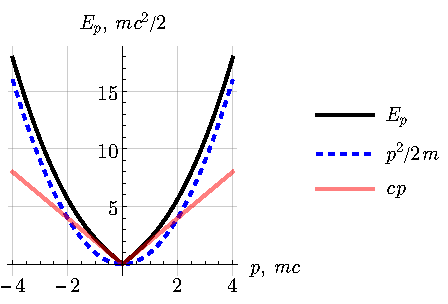
\includegraphics{imgs/MB71.pdf}
    \hspace{10 mm} 
    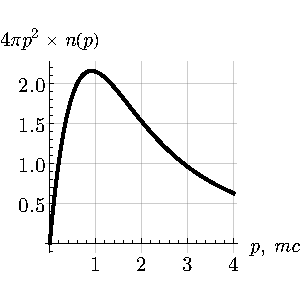
\includegraphics{imgs/MB72.pdf}
    \caption{Exitation energy $E_p$ and the momentum distribution function in 3D $4 \pi p^2 n(p)$}
    \label{fig:MB712}
\end{figure}


\textbf{4. Large canonical ensemble}. In zero order ($N_0 \approx N$) we have $\hat{H} - \mu \hat{N} = - \mu N + \frac{N^2}{2V}\varphi$, thus $\Omega_0 = \bk{\psi}[\hat{H}- \mu \hat{N}]{\psi} \to \min $ and 
\begin{equation*}
	\mu = \varphi n,
\end{equation*}
and we get $\Omega_0 = - \frac{N^2}{2V} \varphi$, so pressure is $P_0 = - \Omega_0 /V$ and hydrodynamic speed of sound
\begin{equation*}
	c^2 = \frac{\partial P_0}{\partial \rho} = V \frac{\partial }{\partial (m N)} \left(- \frac{\Omega_0}{V}\right) = \frac{n \varphi}{m},
\end{equation*}
so we could  rewrite $E_p$ as
\begin{equation}
	E_p = \sqrt{\left(\frac{p^2}{2m}\right)^2 + (cp)^2},
	\hspace{1cm} \Rightarrow \hspace{1cm}
	E_p = \left\{\begin{aligned}
	    &p^2 / 2m, &|p| \gg mc, \\
	    &c |p| , &|p| \ll mc.
	\end{aligned}\right.
\end{equation}
In the long-wave limit, the excitation spectrum has an acoustic character, and the calculated energy deviates from the linear law towards higher energies (fig. \ref{fig:MB712}).


\textbf{5. Ground state and compressibility}. Using \eqref{HBT} and \eqref{Ap} we could calculate the ground state energy
\begin{equation}
	\bk{0}[\hat{H} - \mu \hat{N}]{0} = \Omega_0 = - \mu N + \frac{N^2}{2V}\varphi +\frac{1}{2} \sum_{p \neq 0} (E_p - \epsilon_p).
	\label{BECgs}
\end{equation}
Yes, $\sum_{p \neq 0} (E_p - \epsilon_p)$ diverges as $E_p - \epsilon_p \approx - m n_0^2 \varphi^2 / p^2$ at $p \gg mc$, but for now we will ignore this and find 
\begin{equation*}
	\Omega_0 = - \frac{V}{2\varphi} \mu^2 - \sum_{p > 0} \left(
		\varepsilon_p + \mu - \sqrt{\varepsilon_p^2 - 2 \varepsilon_p \mu} 
	\right)
\end{equation*}
with $N = \mu V  / \varphi$, $n = \mu / \varphi$. Isothermal compressibility is equal
\begin{equation*}
	\kappa = - \frac{1}{V} \frac{\partial^2 \Omega}{\partial \mu^2} = \frac{1}{\varphi} + \frac{1}{V} \sum_{p > 0} \frac{\sqrt{\varepsilon_p}}{(\varepsilon_p -2\mu)^{3/2}},
	\hspace{0.5cm} \Rightarrow \hspace{0.5cm}
	\lim_{\varphi \to 0} \kappa = +\infty,
\end{equation*}
corresponding to the limit of the ideal Bose gase. 


% \textbf{Isothermal compressibility}. 

\textbf{6. Non-condensate particles}.  Now we could express explicitly the number of non-condensate particles by $u$-$v$ Bogoliubov transformation $\langle \hat{a}\D_p \hat{a}_p \rangle = \langle \hat{\alpha}_p\D \hat{\alpha}_p\rangle + v_p^2$. Statistical distribution of elementary excitations $\langle \hat{\alpha}_p\D \hat{\alpha}_p\rangle$ with $T \neq 0$ is given by the Bose distribution with $\mu=0$
\begin{equation*}
	\langle \hat{\alpha}_p\D \hat{\alpha}_p\rangle = \frac{1}{e^{\beta E_p}-1}.
\end{equation*}
With $T=0$
\begin{equation*}
	n(p) =  \langle \hat{a}_p\D \hat{a}_p \rangle = v_p^2 =  \frac{ m^2 c^4}{2 E_p \left(
		E_p + m c^2 + \frac{p^2}{2m}
	\right)}.
\end{equation*}
The total number of non-condensate particles at $T=0$ is (3D case)
\begin{equation*}
	N- N_0 = \frac{V}{(2\pi \hbar)^3} \int_{0}^{\infty}  4 \pi p^2 \d p  \langle \hat{a}_p\D \hat{a}_p \rangle = N \sqrt{n} \frac{(m \varphi)^{3/2}}{3 \pi^2 \hbar^3},
\end{equation*}
and  corresponding <<quantum depletion>> of the condensate
\begin{equation*}
	\frac{N-N_0}{N} = \sqrt{n} \frac{(m \varphi)^{3/2}}{3 \pi^2 \hbar^3}.
\end{equation*}
Inserting\footnote{
	I am not sure about it, but $[\varphi]= [a/m] \cdot [\hbar]^2$ according to the \eqref{BECbase}, that's why wrote $\varphi$ in this way.
} $u=\frac{4\pi a}{m} \hbar^2$, $a=5\,$nm and $n = 10^{20}\,$m${}^{-3}$ (typical values for an ultracold atom experiment with ${}^{87}$Rb) 
\begin{equation*}
	(2\pi \hbar)^3 \frac{N-N_0}{N} \approx 5 \cdot 10^{-2},
\end{equation*}
which justifies the approximation used.




\newpage
\setcounter{section}{8}
% \section{A double well and vortices}
\setcounter{subsection}{0}
\subsection{Effective action of a condensate in a double well}
The following Hamiltonian is a simple model of a condensate in two wells:
\begin{equation}
	H = - \frac{g}{2} \sum_{\langle i,j\rangle} a_i\D a_j + \frac{U}{4} \sum_{j} n_j (n_j-1),
\end{equation}
with $j \in \{1,2\}$. Consider a system with in total $2N$ particles. After normal ordering $[a_i, a_j\D]=\delta_{ij}$
\begin{equation*}
	H(a\D, a) = - \frac{g}{2} \sum_{\langle i,j\rangle} a_i\D a_j  + \frac{U}{4} \sum_{j} a_j\D a_j\D a_j a_j.
\end{equation*}


\textbf{Non-interacting case}. Let's start with $U=0$ and operator canonical transformation (Fourier transform)
\begin{equation*}
	\begin{pmatrix}
		a_1 \\ a_2
	\end{pmatrix} = \begin{pmatrix}
	    \cos \alpha & \sin \alpha \\
	    - \sin \alpha & \cos \alpha \\
	\end{pmatrix} 
	\begin{pmatrix}
		b_1 \\ b_2
	\end{pmatrix},
\end{equation*}
which automatically satisfies the commutation relations $[a_j, a_j\D] = \sin (\alpha)^2 + \cos (\alpha)^2 = 1$. Substituting into the Hamiltonian, we find the condition for diagonalization
\begin{equation*}
	\cos (\alpha)^2 - \sin(\alpha)^2 = 0,
	\hspace{0.5cm} \overset{\alpha=\pi/4}{\Rightarrow}  \hspace{0.5cm}
	a_{1,2} = \tfrac{1}{\sqrt{2}}(b_1 \pm b_2),
\end{equation*}
and the Hamiltonian
\begin{equation}
	H = - \frac{g}{2} \sum_{\langle i,j\rangle} a_i\D a_j =  \tfrac{g}{2} b\D_1 b_1 - \tfrac{g}{2} b\D_2 b_2,
	\label{eq1212}
\end{equation}
with ground state $\ket{0,2N}_b$. Define $\ket{n}_b \overset{\mathrm{def}}{=} \ket{n,2N-n}_b$. Now let's find the $\delta N$ as
\begin{align*}
	\delta N &= a_2\D a_2 - a_1\D a_1 = - b_2\D b_1 - b_1\D b_2,\\
	(\delta N)^2 &= b_1\D b_1 + b_2\D b_2 + 2 b_2\D b_1\D b_1 b_2 = 2N + 4 nN - 2n^2.
\end{align*}
We immediately see that in the ground state 
\begin{equation}
	\langle \delta N^2\rangle_{\text{gs}} = 2N.
	\label{eq2}
\end{equation}
Note that the temperature correction will be
\begin{equation*}
	\tfrac{1}{N} \langle \delta N^2\rangle = 2 \cth\left(\tfrac{1}{2} \beta g\right) \approx 2 + 4 e^{- \beta g}.
\end{equation*}
To calculate this we can start with the partition function
\begin{equation*}
	Z = \sum_{n=0}^{2N} e^{-\beta E_n} = \frac{e^{\beta g (N+1)}-e^{- \beta g N}}{e^{\beta g}-1},
\end{equation*}
with $E_n = - g(N-n)$, and find $\langle n\rangle$ and $\langle n^2\rangle$ through
\begin{equation*}
	\langle N-n\rangle = \frac{1}{\beta} \frac{1}{Z} \frac{\partial Z}{\partial g} = T \partial_g \ln Z,
	\hspace{10 mm} 
	\langle (N-n)^2\rangle = \frac{1}{\beta^2} \frac{1}{Z} \frac{\partial^2 Z}{\partial g^2}.
\end{equation*}



\textbf{Imaginary-time action}. The imaginary-time action associated with this Hamiltonian in the coherent state representation
\begin{equation*}
	S = \tauint \bar{\psi} \partial_\tau \psi + H(\bar{\psi}, \psi)
	=  \tauint 
		\bar{\psi} \partial_\tau \psi - \frac{g}{2} \sum_{\langle i,j\rangle} \bar{\psi}_i \psi_j + \frac{U}{4} \sum_j \bar{\psi}_j \bar{\psi}_j \psi_j \psi_j.
\end{equation*}
Consider the density-phase representation given by
\begin{equation*}
	\psi_1 = \sqrt{N + \frac{\delta N}{2}} e^{i \varphi_1},
	\hspace{10 mm} 
	\psi_2 = \sqrt{N - \frac{\delta N}{2}} e^{i \varphi_2}.
\end{equation*}
The action than
\begin{equation}
	S \overset{\mathrm{def}}{=} \tauint \mathcal{L(\varphi, \theta)} = \tauint 2N i \dot{\theta} + \frac{\delta N}{2} i \dot{\varphi} - g \sqrt{N^2 - \left(\frac{\delta N}{2}\right)^2} \cos \varphi + 2 \frac{U}{4} \left(\frac{\delta N}{2}\right)^2 + \frac{U}{2} N^2  ,
	\label{eqfull}
\end{equation}
with $\varphi = \varphi_1 - \varphi_2$ and $\theta = \tfrac{1}{2}(\varphi_1 + \varphi_2)$. We can find the physical observables that are canonical conjugates to $\varphi$ and $\theta$
\begin{equation*}
	P_\varphi = \frac{\partial \mathcal{L}}{i \partial \dot{\varphi}} = \frac{\delta N}{2},
	\hspace{10 mm} 
	P_\theta = \frac{\partial \mathcal{L}}{i \partial \dot{\theta}} = 2 N,
\end{equation*}
with $i$ factor from Wick rotation $\tau \to - i t$ (it seems to me). 

We can immediately see from Noether’s theorem how symmetry in $\theta$ leads to conservation of $P_\theta = 2N = \const$. And indeed $\mathcal{L}(\theta) = \mathcal{L}(\theta + \text{shift})$ -- $U(1)$ symetry. On the other hand $\mathcal{L}(\varphi) \neq \mathcal{L}(\varphi+\text{shift})$, which corresponds to non-conservation of the $P_\varphi = \delta N$.

\textbf{Effective action}. Expanding the action to quadratic order in the particle number fluctuations $\delta N / N$ and the relative phase $\varphi$ and neglecting constant terms
\begin{equation*}
	\sub{S}{eff}(\varphi, P_\varphi) = \tauint i P_\varphi \partial_\tau \varphi + \tfrac{1}{2} g N\varphi^2 + \tfrac{1}{2}(U + g / N)P_\varphi^2.
\end{equation*}
The fluctuations of the relative particle number
between the wells $(\delta N)^2$ could be found as previous through the partition function $Z$
\begin{equation*}
	Z = \int D[\varphi, P_\varphi] e^{-\sub{S}{eff}(\varphi, P_\varphi)} , 
	\hspace{10 mm} 
	\langle P_\varphi^2\rangle = \frac{1}{Z} \int D[\varphi, P_\varphi]\, P_\varphi^2 e^{-\sub{S}{eff}[\varphi, P_\varphi]} = -\frac{2}{\beta Z} \partial_U Z = -\frac{2}{\beta} \frac{\partial \ln Z}{\partial U},
\end{equation*}
so in what follows we only look at factors containing $U$. Integrating by parts
\begin{equation*}
	\tauint  P_\varphi i \partial_\tau \varphi = P_\varphi i  \varphi \bigg|_{0}^{\beta} - \tauint \varphi i \partial_\tau P_\varphi,
\end{equation*}
and $D[\varphi]$ could be calculated as gaussian integral
\begin{equation*}
	Z \propto \int D[P_\varphi] \exp
	\left(	\tauint 
					\left(- \frac{(\partial_\tau P_\varphi)^2}{2 g N} + \frac{1}{2}(U+g/ N) P_\varphi^2\right)
				\right),
\end{equation*}
that could be calculated in Matsubara representation $2 P_\varphi = \delta N = \frac{1}{\sqrt{\beta}} \sum_k e^{i \omega_k \tau}  \delta N_k $
\begin{equation*}
	Z \propto \int D[\delta N_k] \exp\left(
		- \frac{1}{8}\sum_k \left(
			\frac{\omega_k^2}{gN} + U + \frac{g}{N}
		\right) \delta N_k \delta N_{-k}
	\right).
\end{equation*}
Since the fluctuation $\delta N$ is real, then $\delta N_{-k} = \overline{\delta N}_k$, and
\begin{equation*}
	Z \propto \prod_{k}^{} \left(
		\frac{\omega_k^2}{gN} + U + \frac{g}{N}
	\right)^{-1/2}
	\hspace{0.5cm} \Rightarrow \hspace{0.5cm}
	\langle \delta N^2\rangle = \frac{4}{\beta} \sum_k \left(\frac{\omega_k^2}{gN} + U + \frac{g}{N}\right)^{-1},
\end{equation*}
with $\omega_k = 2 \pi k / \beta $. After summation as
\begin{equation*}
	\sum_{k=-\infty}^{\infty} \frac{1}{k^2 + x^2} = \frac{\pi}{x} \frac{1}{\cth (\pi x)},
	\hspace{0.5cm} \Rightarrow \hspace{0.5cm}
	\langle \delta N^2\rangle = 2 N \frac{\cth \left(\tfrac{1}{2} \beta g F_U \right)}{F_U},
\end{equation*}
with $F_U = \sqrt{1 + NU/g}$, in full accordance with formula \eqref{eq2}.



\textbf{Low fluctuations}. The expansion in $\delta N / N$ is
justified with  $|\delta N| / N \ll 1$ or $\cth \left(\tfrac{1}{2} \beta g F_U \right) / N F_U \ll 1$. Note that temperature increases fluctuations and decreases interaction. Thus  we could rewrite \eqref{eqfull} as
\begin{equation*}
	\sub{S}{eff}(\varphi, P_\varphi) = \tauint P_\varphi i \partial_\tau \varphi - g N \cos(\varphi) + \tfrac{1}{2} U P_\varphi^2,
\end{equation*}
where we neglected $P_\varphi^2 / N$ term. 


\textbf{Equations of motion}. The real-time effective action is
\begin{equation*}
	\sub{S}{eff}[\varphi, P_\varphi] = i \int_{0}^{T} \hspace{-1mm} d t\ \mathcal{L} = i \int_{0}^{T} \hspace{-1mm} d t\  \left(P_\varphi \partial_t \varphi + g N \cos (\varphi) - \tfrac{1}{2} U P_\varphi^2\right).
\end{equation*}
Classical equations of motion could be obtained from Euler–Lagrange equation
\begin{equation*}
	\frac{\partial \mathcal{L}}{\partial x} - \frac{d }{d t} \frac{\partial \mathcal{L}}{\partial \dot{x}} = 0,
	\hspace{0.5cm} \Rightarrow \hspace{0.5cm}
	\left.\begin{aligned}
	    \dot{\varphi} &= U P_\varphi, \\
	    \dot{P}_\varphi &= - g N \sin(\varphi)
	\end{aligned}\right.
	\hspace{0.5cm} \Rightarrow \hspace{0.5cm}
	\partial_t^2 \varphi = - g N U \sin \varphi.
\end{equation*}
The current between the wells is $\partial_t \delta N / 2 = \partial_t P_\varphi = - g N \sin \varphi$, limited by $g N$.


\textbf{Oscillation frequency}. With $\varphi_0 \ll 1$ we could limit $|\varphi|$ and rewrite equations as
\begin{equation*}
	\ddot{\varphi} = g N U \varphi,
	\hspace{1cm} \Rightarrow \hspace{1cm}
	\varphi = \varphi_0 \cos(\sqrt{gNU} t),
\end{equation*}
so oscillation frequency is $\sqrt{g N U}$. Fluctuations are also small as $P_\varphi = \dot{\varphi}/U$. Non-interacting bosons oscillation could be found from \eqref{eq1212} with $\ket{\psi(t)} = \sum_{n=0}^{2N} \alpha_n e^{i g (N-n) t} \ket{n,2N-n}$, we obtain
\begin{equation*}
	\langle \delta N(t)\rangle = \bk{\psi(t)}[- b_2\D b_1 - b_1\D b_2]{\psi(t)} = \bra{\psi(t)} \sum_{n=1}^{2N-1} \sqrt{n(2N-n-1)} \alpha_n  e^{i g (N-n)t}\ket{n,2N-n} e^{-i g t} = \sum_n ... e^{-igt},
\end{equation*}
so oscillation frequency is $g$.




% \begin{equation*}
% 	\sub{k}{B} \sub{k}{F} \sub{\mu}{B} 
% \end{equation*}



\newpage
\subsection{Vortex Excitation in a Superfluid}




\newpage
\setcounter{section}{10}
% \section{Introduction to Landau’s Fermi Liquid Theory}
\setcounter{subsection}{0}
\subsection{Phase Space Argument for the Life Time of Quasi-particles}


\textbf{1. Exact expression}.
Consider the Coulomb interaction in second quantization between electrons:
\begin{equation*}
	\blue{\hat{V}} = \frac{1}{2 \mathcal{V}} \sum_{\sigma \sigma'} \sum_{k k' q} V(q) 
	\blue{c\D_{k + q,\sigma} c\D_{k'-q,\sigma'} c_{k', \sigma'} c_{k, \sigma}},
\end{equation*}
$\mathcal{V}$ is the volume. Taking into account only scattering processes that involve two
particles, we could derive an expression for the inverse life time $1/ \tau_k$ of the state\footnote{
	Here and further $\overset{\mathrm{n}}{=}$ means that we ignore normalization factor, that appears in $\mathcal{N}_{i,f}$.
} $\ket{i} = \ket{k_1, \sigma_1} \overset{\mathrm{n}}{=}  c\D_{k_1, \sigma_1} \ket{\Omega}$, where $\ket{\Omega}$ denotes the state, where all states below Fermi surface are occupied. 


With Fermi's Golden Rule (fig. \ref{fig:absd}b)
\begin{equation*}
	\frac{1}{\tau_{k_1}} = 2 \pi \sum_{f} |\bk{f}[\blue{\hat{V}}]{k, \sigma}|^2 \delta(\varepsilon_i - \varepsilon_f),
	\hspace{10 mm}
	\ket{f} \overset{\mathrm{n}}{=}  c\D_{k_1-Q,\sigma_1} c\D_{k_2+Q,\sigma_2} c_{k_2,\sigma_2} \ket{\Omega}. 
\end{equation*}
Thus life time could be expressed from the matrix elements
\begin{equation*}
% \bk{k_1, \sigma_1} [\blue{\hat{V}}]{k_1-Q,\sigma_1; k_2+Q,\sigma_2; \cancel{k_2, \sigma_2}} 
\bk{i} [\blue{\hat{V}}]{f} 
= 
\frac{1}{2 \mathcal{V}} \sum_{\sigma \sigma'} \sum_{k' q} \mathcal{N}_{i,f} V(q) 
	\bk{\Omega}[
		c_{k_1, \sigma_1}  
		\blue{c\D_{k + q,\sigma} c\D_{k'-q,\sigma'} c_{k', \sigma'} c_{k, \sigma}}   
		c\D_{k_1-Q,\sigma_1} c\D_{k_2+Q,\sigma_2} c_{k_2,\sigma_2}
	]{\Omega},
\end{equation*}
with normalizing factor 
\begin{equation*}
	\mathcal{N}_{i,f} = \left(
		(1- n_{k_1, \sigma_1})(1- n_{k_1-Q, \sigma_1}) (n_{k_2, \sigma_2})(1- n_{k_2+Q, \sigma_2})
	\right)^{-1/2},
\end{equation*}
since $\langle c\D c\rangle = n$ and $\langle c c\D\rangle = 1-n$.


\begin{figure}[h]
    \centering
    \vspace{-10mm}
    \addletter{80}{a} \hspace{5 mm} 
    \begin{tikzpicture}
	\begin{feynman}[large]
		\vertex (i1);
		\vertex [below right=of i1] (a);
		\vertex [below left=of a] (i2);
		\vertex [right=of a] (b);
		\vertex [above right=of b] (f1);
		\vertex [below right=of b] (f2);
		\diagram* {
		(i1) -- [fermion, edge label=\(k\,\sigma\)] (a) -- [fermion, edge label=\(k+q\,\sigma\)] (i2),
		(f1) -- [fermion, edge label'=\(k'\,\sigma'\)] (b) -- [fermion, edge label=\(k'-q\,\sigma'\)] (f2),
		(a) -- [boson] (b),
		};
	\end{feynman}
	\end{tikzpicture}
	\hspace{10 mm} 
	\addletter{80}{b}
    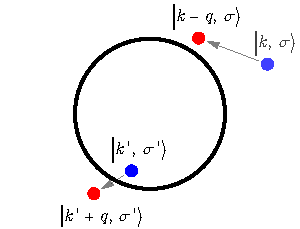
\includegraphics{imgs/FSe.pdf}
    \caption{Scattering process}
    \label{fig:absd}
\end{figure}

% Осталось подружить друг с другом состояния.
To calculate this matrix element we need just to decide how to distribute $\ket{k_1, \sigma_1}$, $\ket{k_2, \sigma_2}$, $\ket{k_1-Q, \sigma_1}$, $\ket{k_2+Q, \sigma_2}$ over the $\ket{k, \sigma}$, $\ket{k', \sigma'}$, $\ket{k'-q, \sigma'}$, $\ket{k+q,\sigma}$ (fig. \ref{fig:absd}a). There are only two different ways to do this (\red{sign} could be found as in the Wick's theorem):
\begin{align*}
	% \bk{k_1, \sigma_1} [\blue{\hat{V}}]{k_1-Q,\sigma_1; k_2+Q,\sigma_2; \cancel{k_2, \sigma_2}} = 
	\bk{i}[\hat{V}]{f}_1 
	&= 
	\frac{\mathcal{N}_{i,f}}{2\mathcal{V}} \sum_{k,k',q} \sum_{\sigma_1,\sigma_2} V(q)   \delta_{\sigma_1, \sigma} \delta_{\sigma_2, \sigma'} \delta(k_1-k-q)  \delta(Q-q) (1-n_{k_1}) n_{k_2} (1-n_{k_1-Q}) (1-n_{k_2+Q})
	\\ &= 
	\frac{\mathcal{N}_{i,f}}{2\mathcal{V}} V(Q) (1-n_{k_1, \sigma_1}) n_{k_2,\sigma_2} (1-n_{k_2+Q,\sigma_2})(1-n_{k_1-Q,\sigma_1})
	,
\end{align*}
and
\begin{align*}
	\bk{i}[\hat{V}]{f}_2 = \ldots
	% \red{-}\mathcal{N}_{i,f}\sum_{k,k',q} \sum_{\sigma_1,\sigma_2}V(q) \delta_{\sigma_1, \sigma} \delta_{\sigma_2, \sigma'} \delta(k_1-k-q)  \delta(k_2-k'+q) \delta(Q-q) (1-n_{k_1}) n_{k_2} (1-n_{k_1-Q}) (1-n_{k_2+Q}) 
	= \red{-} \frac{\mathcal{N}_{i,f}}{2\mathcal{V}} V(k_1-k_2-Q) \delta_{\sigma_1, \sigma_2} 
	(1-n_{k_1,\sigma_1} )
	n_{k_2,\sigma_2}
	(1-n_{k_2+Q,\sigma_2})
	(1-n_{k_1-Q,\sigma_1})
	.
\end{align*}
Due to symmetry, each term will appear twice, which means
\begin{equation*}
	\bk{i}[\hat{V}]{f} = \frac{\mathcal{N}_{i,f}}{\mathcal{V}} V(Q) (1-\delta_{\sigma_1,\sigma_2}) (1- n_{k_1, \sigma_1})(1- n_{k_1-Q, \sigma_1}) (n_{k_2, \sigma_2})(1- n_{k_2+Q, \sigma_2}) = \frac{1-\delta_{\sigma_1,\sigma_2}}{\mathcal{V} \mathcal{N}_{i,f}} V(Q).
\end{equation*}
As expected, we found that only particles with different spins are scattered.


Let's move on to integration
\begin{equation*}
	\frac{1}{\tau_{k_1}} 
	= 
	2 \pi \sum_{f} |\bk{f}[\blue{\hat{V}}]{k, \sigma}|^2 \delta(\varepsilon_i - \varepsilon_f) 
	= 
	\frac{2\pi}{\mathcal{V}^2} \int \frac{d^3 k_2\ d^3 Q}{(2\pi)^6} |V(Q)|^2 \mathcal{N}_{i,f}^{-2}
	\delta(\varepsilon_i - \varepsilon_f) \sum_{\sigma_2} (1-\delta_{\sigma_1,\sigma_2}),
\end{equation*}
with $\varepsilon_i - \varepsilon_f = \varepsilon_{k_1} - \varepsilon_{k_1-Q} - \varepsilon_{k_2+Q} + \varepsilon_{k_2}$.


% kkhoruzhii
% 256494936Fermi!




\textbf{2. Approximate calculation}. 
By anticipating the result for the screening of the Coulomb interaction, we can
assume that  $V(Q) \approx V(0) = \const$. It is convenient to use  (with $\xi = \varepsilon - \varepsilon_F$ and $d \vc{k} = d \cos \theta \, d \varphi$)
\begin{equation*}
	\int \frac{d^3 k}{(2\pi)^3} 
	= \int \frac{d \vc{k}}{4\pi} \int d\xi \, N(\xi)  
	=  N(0)\int \frac{d \vc{k}}{4\pi} \int \d \xi
	.
\end{equation*}
We consider system at $T=0$:
\begin{equation*}
	(1- n_{k_1, \sigma_1})(1- n_{k_1-Q, \sigma_1}) (n_{k_2, \sigma_2})(1- n_{k_2+Q, \sigma_2}) = \theta(\xi_{k_1}) \theta(- \xi_{k_2}) \theta(\xi_{k_1-Q}) \theta(\xi_{k_2+Q}).
\end{equation*}
Substituting this into the expression for the lifetime, we find
\begin{equation*}
	\frac{1}{\tau_{k_1}} \approx \frac{2\pi}{\mathcal{V}^2} |N(0)|^2 V(0)^2
	\int d \xi_{k_2} 
	\int \frac{d \vc{k}_{k_2}}{4\pi} 
	\int d \xi_{Q} 
	\int \frac{d \vc{k}_{Q}}{4\pi} 
	\theta(\xi_{k_1}) \theta(- \xi_{k_2}) \theta(\xi_{k_1-Q}) \theta(\xi_{k_2+Q})
	\delta( \varepsilon_{k_1} - \varepsilon_{k_1-Q} - \varepsilon_{k_2+Q} + \varepsilon_{k_2}).
\end{equation*}
Let's define $k_f = k_1 - Q$. As in the fig. \ref{fig:absd}b we take $\xi_{k_1} > 0$ and $\xi_{k_2+Q} > 0$
 % and $\xi_{k_f} < `$
\begin{equation*}
	\delta( \varepsilon_{k_1} - \varepsilon_{k_f} - \varepsilon_{k_1+k_2-k_f} + \varepsilon_{k_2}) = \frac{1}{2 \varepsilon_F} \delta\left(
		1 + \tilde{\vc{k}}_1 \cdot \tilde{\vc{k}}_2 - \tilde{\vc{k}}_1 \cdot \tilde{\vc{k}}_f - \tilde{\vc{k}}_2 \cdot \tilde{\vc{k}}_f
	\right),
\end{equation*}
with $\tilde{\vc{k}} = \vc{k} / k$. Rewriting the integral for the last time
\begin{equation*}
	\frac{1}{\tau_{k_1}} \approx  \frac{2\pi}{\mathcal{V}^2} |N(0)|^2 V(0)^2 \int_{-\xi_{k_1}}^{0} d \xi_{k_2} \int_{0}^{\xi_{k_1}-\xi_{k_2}} d \xi_{k_f} 
	\int \frac{d \vc{k}_{k_2}}{4\pi} \int \frac{d \vc{k}_{Q}}{4\pi} 
	\frac{1}{2 \varepsilon_F} \delta\left(
		1 + \tilde{\vc{k}}_1 \cdot \tilde{\vc{k}}_2 - \tilde{\vc{k}}_1 \cdot \tilde{\vc{k}}_f - \tilde{\vc{k}}_2 \cdot \tilde{\vc{k}}_f
	\right),
\end{equation*}
so finally
\begin{equation*}
	\frac{1}{\tau_{k_1}} \propto (\varepsilon_{k_1}-\varepsilon_F)^2.
\end{equation*}
\subsection{Microscopic Basis of the Fermi-liquid Theory}
Fermi liquid theory only holds if the ground state of the interacting
system is connected adiabatically to the non-interacting Fermi sea. One can treat this
as turning on the interactions adiabatically. The ground state $\gs$ of the full system and
the excitation state $\blue{\ket{\vc{k}, \sigma}}$ can then be written as
\begin{equation*}
	\gs = U \ket{\Omega},
	\hspace{10 mm} 
	\blue{\ket{\vc{k}, \sigma}} = U \ket{\vc{k}, \sigma} = U c\D_{\vc{k},\sigma} \ket{\Omega}.
\end{equation*}
The time evolution operator in the interaction picture can be
expressed as a time-ordered exponential
\begin{equation*}
	U = T\left\{
		e^{- i \int_{-\infty}^{0} \hat{V}(t) \d t}
	\right\}.
\end{equation*}
The quasi-particle creation operator (№3) could be expressed from the 
\begin{equation*}
	\blue{\ket{\vc{k}, \sigma}} = a\D_{\vc{k}, \sigma} \gs = U c\D_{\vc{k}, \sigma} \ket{\Omega} = U c\D_{\vc{k}, \sigma} U^{-1} \ket{\varphi},
	\hspace{0.5cm} \Rightarrow \hspace{0.5cm}
	a\D_{\vc{k}, \sigma} = U c\D_{\vc{k}, \sigma} U^{-1}.
\end{equation*}

For Fermi liquid theory to be valid, one need to add requirement on
the wavefunction renormalization constant
\begin{equation*}
	Z_k = |\bk{\blue{k \sigma}}[c\D_{k \sigma}]{\text{gs}}|^2 = |\bk{\text{gs}}[a_{k\sigma} c\D_{k \sigma}]{\text{gs}}|^2 .
\end{equation*}
Expressing $c\D_{k \sigma}$ as a series in the quasi-particle operators
\begin{align*}
	c\D_{k \sigma} &= U\D a\D_{k \sigma} U \approx \left(
		1 + i \int_{-\infty}^{0} \hat{V}(t) \d t
	\right) a\D_{k \sigma} \left(1 - i \int_{-\infty}^{0} \hat{V}(t) \d t\right) = a\D_{k \sigma} + i \int_{-\infty}^{0} [\hat{V}(t), a\D_{k\sigma}] \d t + O(V^2) \\
	&= \sqrt{Z_k} a\D_{k \sigma} + \text{higher order}
\end{align*}
If we want to $c_{k \sigma}\D \approx a_{k \sigma}\D$, then (№4) $0 < \sqrt{Z_k} < 1$.


The spectral function (fig. \ref{fig:Apeak})
\begin{equation*}
	A(k, \omega) = - \frac{1}{\pi} \Im G^{\text{ret}} (k, \omega) = \sum_\lambda |M_\lambda|^2 \delta(\omega-\xi_\lambda),
	\hspace{10 mm} 
	|M_\lambda|^2 = |\bk{\lambda}[c\D_{k, \sigma}]{\text{gs}}|^2
\end{equation*}
exhibits a sharp quasiparticle peak at $\xi_k$
\begin{equation*}
	A(k, \omega) = Z_k \delta(\omega - \xi_k) + \ldots
\end{equation*}
with $Z_k > 0$. Thus momentum distribution $\langle \hat{n}_{k \sigma}\rangle$  has a jump at the Fermi momentum
\begin{equation*}
	\langle \hat{n}_{k \sigma}\rangle = \bk{\text{gs}}[c\D_{k \sigma} c_{k \sigma}]{\text{gs}} =
 \int A(k, \omega) n_f(k, \omega) \d \omega = \int Z_k \delta(\omega-\varepsilon_k) \theta(\varepsilon_f - \theta)  \d \omega + \ldots 
	= Z_k \theta(\varepsilon_F - \varepsilon_k) + \ldots
\end{equation*}

\begin{figure}[h]
    \centering
    \addletter{60}{a} 
    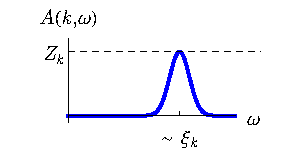
\includegraphics{imgs/Apeak.pdf}
    \hspace{10 mm} 
    \addletter{60}{b} 
    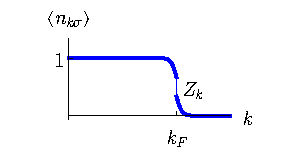
\includegraphics{imgs/npeak.pdf}
    \caption{a) The spectral function. b) The momentum distribution.}
    \label{fig:Apeak}
\end{figure}




\addcontentsline{toc}{subsection}{11.1 \ (external) Fermi Liquid Theory and Green’s Functions}
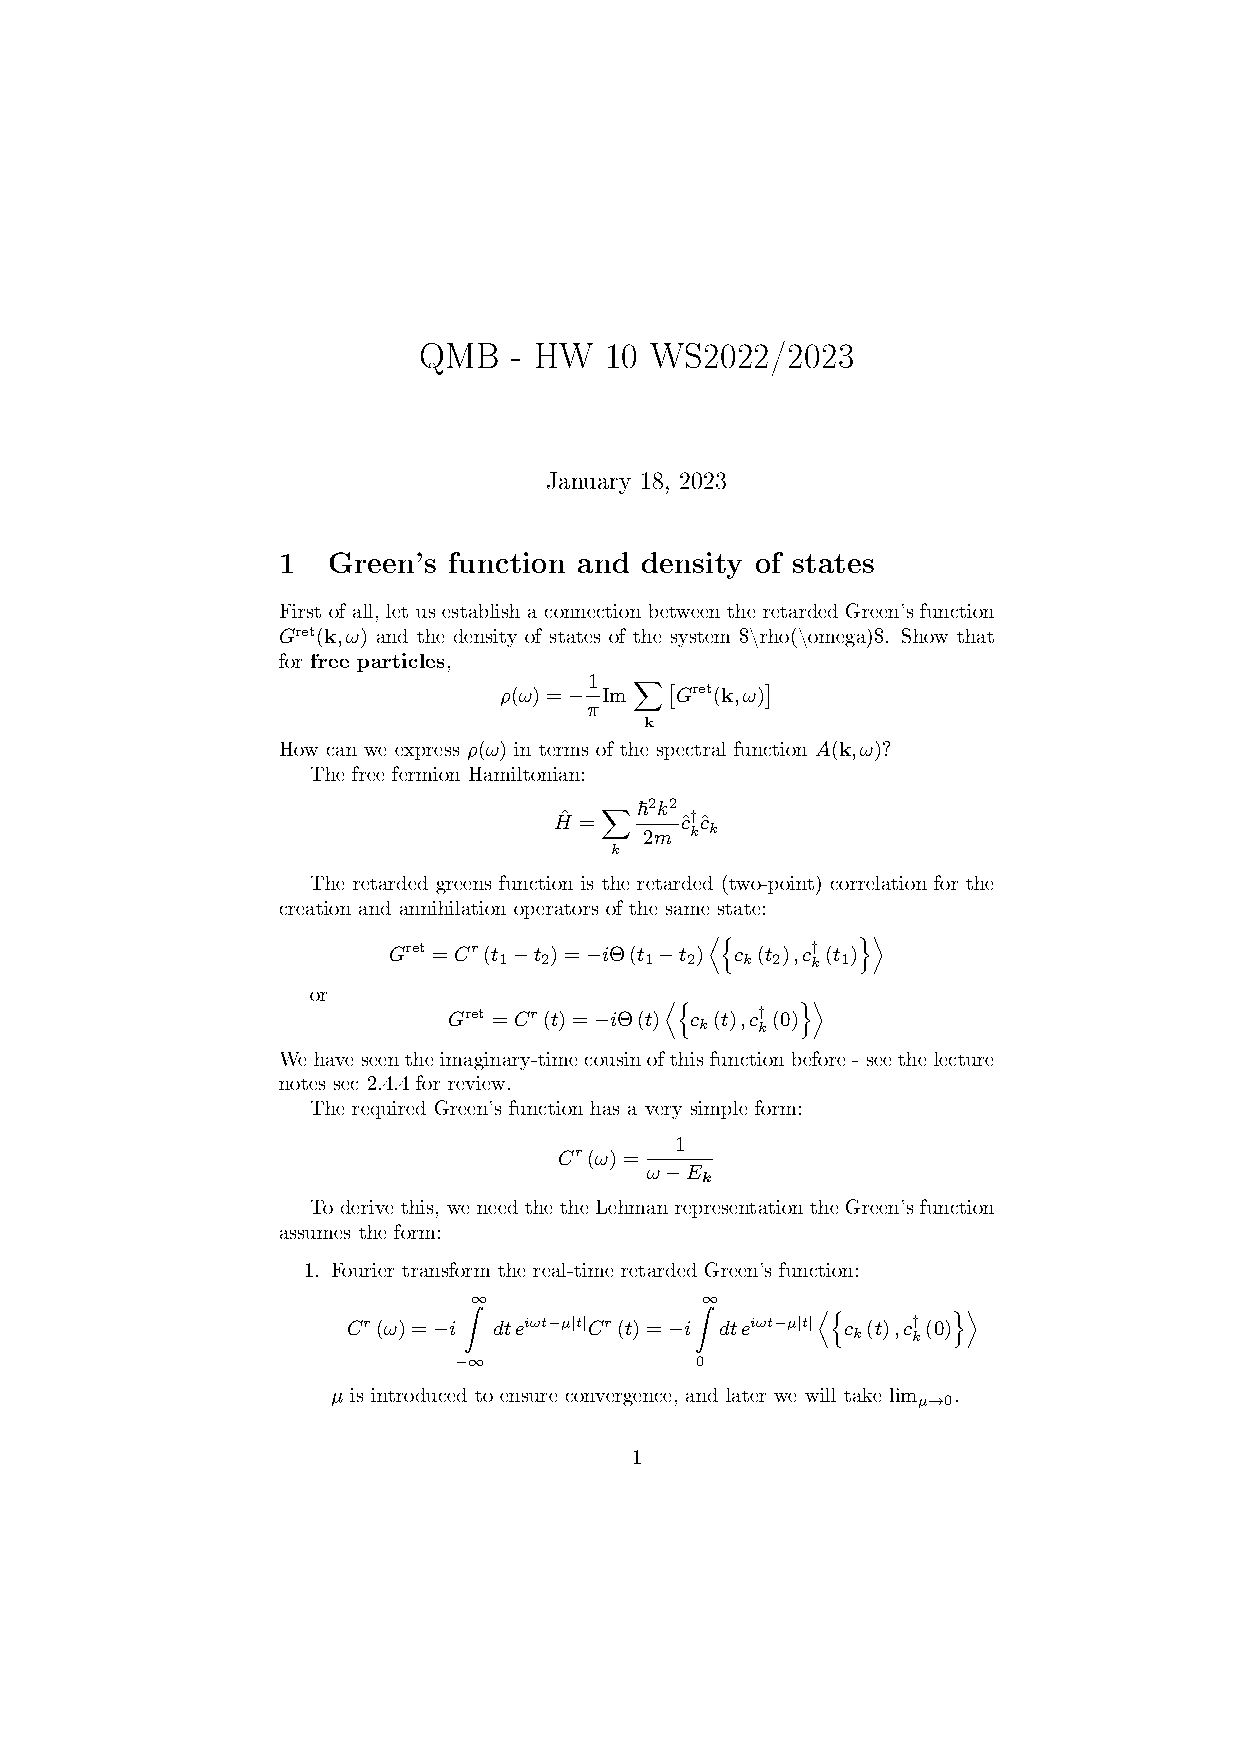
\includepdf[pages=-]{MBs11.pdf}





\setcounter{section}{12}
\setcounter{subsection}{0}
\subsection{Fermions in one dimension}


Consider 1D non-interacting electrons described by the Hamiltonian
\begin{equation*}
	\hat{H} = \sum_k \xi_k \hat{c}_k\D \hat{c}_k,
	\hspace{10 mm} 
	\xi_k = \varepsilon_k - \mu.
\end{equation*}
We want to compute the Linchard function $\chi_0$
is the
correlation function
associated
with the
response
to
a
change
of the
chemical
potential.


\textbf{1. Lindhard function}.  The density response function $\chi_0(q, \omega)$ of a one-dimensional Fermi gas 
\begin{equation*}
	\chi_0(q, t) = - \frac{i}{\hbar} \theta(t) \langle [\hat{\rho}_q(t), \hat{\rho}_{-q} (0)]\rangle,
\end{equation*}
% with thermal expectation value over $\rho = e^{- \beta H} / Z$. Here 
% \begin{equation*}
% 	\hat{\rho}_q \overset{\mathrm{n}}{=}  \sum_k \hat{c}_{k+q}\D \hat{c}_k,
% \end{equation*}
% is the Fourier transform of the density operator $\hat{\rho}_r = \hat{\psi}\D(r) \hat{\psi}(r)$
% \begin{equation*}
% 	\hat{\rho}_q \overset{\mathrm{n}}{=} \int dr \ \hat{\psi}\D(r) \hat{\psi}(r)  e^{- i q r}.
% \end{equation*}
% The time evolution $\hat{\rho}_q$  is given by
% \begin{equation*}
% 	\hat{\rho}_q (t) \overset{\mathrm{n}}{=} \sum_k e^{i (\xi_{k+q}-\xi_k)t} \hat{c}_{k+q}\D \hat{c}_k. 
% \end{equation*}
Thus we find for the Fourier transform of the Lindhard function	
\begin{equation*}
	\chi_0 (q, \omega) = - \frac{i}{\hbar} \int_{-\infty}^{\infty} dt \ 
	e^{i \omega t} \theta(t) \langle [\hat{\rho}_q(t), \hat{\rho}_{-q} (0)]\rangle = - \frac{i}{\hbar V} \sum_k \int_{0}^{\infty} dt\ 
	e^{i(\omega - (\xi_k - \xi_{k+q}))t} \left[
		n_{k+q} (1-n_k) - n_k (1 - n_{k+q})
	\right],
\end{equation*}
where we took advantage of the quadratic Hamiltonian of free fermions. 
\begin{equation*}
	\chi_0 (q, \omega) = \frac{1}{\hbar V} \sum_k \frac{n_{k+q} - n_k}{\omega- (\xi_k - \xi_{k+q}) + 0 i}.
\end{equation*}
% \red{
% If we use other defininiton $\hat{\rho}_q = \sum_k \hat{c}_k \hat{c}_{k+q}$, then
% \begin{equation*}
% 	\chi_0 (q, \theta) = \frac{1}{\hbar V} \sum_k \frac{n_{k+q}- n_k}{\omega + (\xi_k - \xi_{j+q}) + 0i}.
% \end{equation*}
% Using that
% \begin{equation*}
% 	\lim_{\eta \to 0} \frac{1}{\omega + i \eta} = \mathcal{P}\left(\frac{1}{\omega}\right) - i \pi \delta(\omega).
% \end{equation*}
% }
Moving on to integration
\begin{equation*}
	\chi_0 (q,\omega) = \frac{1}{V \hbar} \int_{-\infty}^{\infty} \frac{dk}{2\pi} \frac{n_{k+q} - n_k}{\omega- (\xi_k - \xi_{k+q}) + 0 i} = \mathcal{P} \int_{-\infty}^{\infty} \frac{dk}{2\pi} \frac{n_{k+q} - n_k}{\omega- (\xi_k - \xi_{k+q})} - i \pi \int_{-\infty}^{\infty} \frac{dk}{2\pi} 
	\left(n_{k+q} - n_k\right) \delta(\omega - (\xi_{k+q}-\xi_k)),
\end{equation*}
we get
\begin{align*}
	\chi_0''(q,\omega) &= \Im \chi_0 (q, \omega) = \frac{1}{2} \int_{-\infty}^{\infty} dk\ \left(
		\delta(\omega - (\xi_{k+q}-\xi_k)) - \delta(\omega - (\xi_k - \xi_{k-1}))
	\right) n_k 
	\\ &= 
	\frac{m}{2|q|} \int_{-\infty}^{\infty} n_k (\delta(k-k_-) - \delta(k - k_+)) \d k = \frac{m}{2|q|} \left(
		n_{k_-} - n_{k_+}
	\right)
	,
\end{align*}
with defined zeros 
\begin{equation*}
	\delta(\omega - (\xi_{k+q} - \xi_k)) = \frac{m}{|q|} \delta(k - k_\pm),
	\hspace{10 mm} 
	k_{\pm} = \frac{2 m \omega \pm q^2}{2q}.
\end{equation*}


% \newpage
\textbf{2. Perturbation}.  The energy absorption rate $\propto \chi_0 (q, \omega)$ from the perturbation $(q, \omega)$. At zero temperature $\chi_0(T=0)''$ could be rewritten as
\begin{equation*}
	\chi_0''(q,\omega) = \frac{m}{2|q|} \left(
		\theta(- \xi_{k_-}) - \theta(-\xi_{k_+})
	\right),
	\hspace{10 mm} 
	\xi_k = \frac{\hbar^2 k^2}{2m}  - \frac{\hbar^2 \kF^2}{2m},
	\hspace{5 mm} 
	k_{\pm} = \frac{2 m \omega + q^2}{2q},
\end{equation*}
which completely defines regions with non-zero absorption. Let's find conditions for the boundaries (in units of $\kF$ and $\varepsilon_\text{F}$)
\begin{equation*}
	\left\{\begin{aligned}
	    \kF^2 - k_-^2 &> 0 \\
	    \kF^2 - k_+^2 &< 0 \\
	\end{aligned}\right.
	\hspace{0.5cm} \Rightarrow \hspace{0.5cm}
	\left\{\begin{aligned}
	    &q - \frac{1}{2}q^2  < \omega < q + \frac{1}{2} q^2, &0 < q< 2 \\
	    &-q + \frac{1}{2} q^2   < \omega < q + \frac{1}{2} q^2,  &q > 2
	\end{aligned}\right.
\end{equation*}
, which, taking into account symmetry $\chi_0''(q) = \chi_0''(-q)$, leads to (fig. \ref{fig:12_1}). 
Here we see well defined sharp $\omega(q)$ at $q \ll \kF$ (in contrast to 2D/3D case with macroscopic Fermi surface).


\begin{figure}[h]
    \centering
    \addletter{80}{a}
    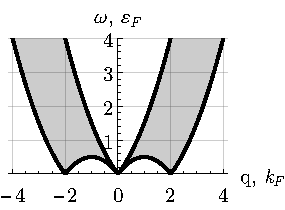
\includegraphics{imgs/mb12_1.pdf}
    \hspace{10 mm} 
    \addletter{80}{b}
	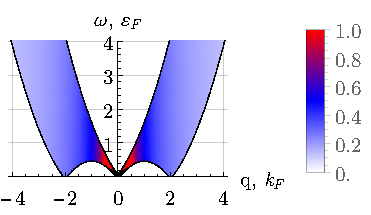
\includegraphics{imgs/mb12_2.pdf}
    \caption{a) Nonzero energy absorption rate regions.  b) The density response function $\chi$ of the weak interacting system. }
    \label{fig:12_1}
\end{figure}



\newpage
\textbf{3.  The sound velocity.} 
The sound velocity of the 1D non-interacting Fermi gas, i.e. the proportionality constant of the linear dispersion at small $q$
\begin{equation*}
	\sub{v}{sound} = \frac{ \hbar \kF}{m}\frac{\partial }{\partial q} \left(q - \tfrac{1}{2} q^2\right) |_{q = 0} = \frac{\hbar \kF}{m} = \sub{v}{F}.
\end{equation*}





\textbf{4. Width.} The width of the region in which energy can be absorbed $\delta \omega (q \ll \kF)$ 
\begin{equation*}
	\delta \omega (q \ll \kF) \approx \varepsilon_\text{F} (q / \kF)^2,
\end{equation*}
so there is  a sharp collective mode in the spectrum
in the sense that 
\begin{equation*}
	\lim_{q \to 0} \frac{\delta \omega (q)}{\omega(q)} = \frac{\varepsilon_\text{F}}{\kF^2}\lim_{q \to 0} \frac{q^2}{\sub{v}{F} q} = 0,
\end{equation*}
and (remembering Luttinger's liquid) operator that create these
excitations on top of the ground-state 
% \begin{equation*}
$
	\hat{\rho}_q,
$
% \end{equation*}
which is specific to one-dimensional systems.

\textbf{5. RPA.} Now we add a contact interaction $u$ between the Fermions. The density response function $\chi(q, \omega)$ of the interacting system at small $q$ at zero temperature, using the result of the random phase approximation (RPA)
\begin{equation*}
	\chi(q, \omega) = \frac{\chi_0(q, \omega)}{1 - u \chi_0 (q, \omega)}.
\end{equation*}

%  While the imaginary part doesn't change much, the real part does
% \begin{equation*}
% 	\chi
% \end{equation*}

To find the pole we need
\begin{align*}
	\chi_0' (q, \omega) &= \Re \int_{-\infty}^{\infty} \frac{dk}{2\pi} \frac{n_{k+q} - n_k}{\omega - ( \xi_{k+q} - \xi_k) + 0 i} 
	\\ &= 
	\Re \int_{-\kF - q}^{\kF - q} \frac{dk}{2\pi} \frac{1}{\omega - \frac{1}{2m} (2 k q + q^2) + i0} - 
	\Re  \int_{-\kF}^{\kF} \frac{dk}{2\pi} \frac{1}{\omega - \frac{1}{2m} (2 k q + q^2) + i0}
	\\ &\approx \frac{1}{\pi} \frac{q^2 \vF}{\omega^2 + \vF^2 q^2}.
\end{align*}
Thus $\xi$ has a pole at $1 - u \chi_0 = 0$ 
\begin{equation*}
	\omega = \sqrt{1+ \tfrac{1}{\pi \vF}} \vF = \sub{\tilde{v}}{sound} q,
	\hspace{10 mm} 
	\sub{\tilde{v}}{sound} = \vF \sqrt{1 + \frac{u}{\pi \vF}},
\end{equation*}
with almost the same the sound velocity.


\textbf{6. On the way to bosonisation}.
The sound-mode exhausts the $f$-sum rule
\begin{equation*}
	\int_{-\infty}^{\infty} \omega S(q, \omega) \d \omega = \frac{q^2}{2m},
\end{equation*}
at zero temperature, i.e. all the excitations of a 1D Fermi system are phonons. The imaginary part
\begin{equation*}
	\chi''(q,\omega) = \frac{\chi_0''}{(1 - u \chi_0')^2 + u^2 (\chi_0'')^2} \overset{ \chi'' \neq 0}{=} \frac{m}{2|q|}  \left(
		 \left(\frac{u m}{2q}\right)^2 + \left(1 - \frac{u}{\pi} \frac{q^2 \vF}{q^2 \vF^2 + \omega^2}\right)^2
	\right)^{-1}.
\end{equation*}
Thus sum rule
\begin{align*}
	\int_{-\infty}^{\infty} \omega S(q, \omega) \d \omega &= 2\int_{-\infty}^{\infty} \omega \chi''(q, \omega) \theta(\omega) \d \omega = \frac{1}{\pi} \int_{0}^{\infty} \omega \chi''(q, \omega) \d \omega.
\end{align*}
We could for example assume $q \ll \kF$ and expand in series of $\omega$
\begin{equation*}
	 \omega \chi''(q, \omega) \approx \frac{m \omega }{2 q \left(\frac{m^2 u^2}{4 q^2}+\left(1-\frac{u}{\pi  v_\text{F}}\right)^2\right)},
\end{equation*}
and
\begin{equation*}
	\int_{-\infty}^{\infty} \omega S(q, \omega) \approx \int_{q - q^2/2}^{q + q^2/2}  \frac{\omega}{2 q} \left(\frac{u^2}{4q^2} + (1-\frac{u}{\pi})^2\right) \approx q^2 \red{\left(
		\frac{u^2}{4 q^2}+\frac{u^2}{\pi ^2}-\frac{2 u}{\pi }+1
	\right)^{-1}},
\end{equation*}
with $m=1$, $\vF=1$.
In general, something like a quadratic. 






















\setcounter{section}{13}
\setcounter{subsection}{0}


\newpage
\subsection{Stoner instability}
Consider a 3D Fermi gas with point-like interactions:
\begin{equation*}
	H = T + V = \sum_{k \sigma} \left(
		\frac{k^2}{2\sub{m}{e}}-\mu
	\right) n_{k \sigma} + u 
	\int \psi\D_{\up} (x) \psi\D_{\down} (x) \psi_{\down} (x) \psi_{\up} (x) \d^3 x,
\end{equation*}
or, completely in the momentum representation:
\begin{equation*}
	H = \sum_{k \sigma} \left(
		\frac{k^2}{2\sub{m}{e}}-\mu
	\right) n_{k \sigma} + \frac{u}{V}  \sum_{k_1, k_2, q} c\D_{k_1 + q, \up} c\D_{k_2 - q, \down} c_{k_2, \down} c_{k_1, \up},
\end{equation*}
after substitution $\psi_\sigma(x) = V^{-1/2} \sum_k e^{- i k x} c_{k, \sigma}$.

\textbf{The density of states}. 
The density of states at the Fermi Energy for the non-interacting system
\begin{equation*}
	2 \int \frac{d^3 k}{(2\pi)^3} = \int d\varepsilon \ D(\varepsilon),
	\hspace{5 mm} 
	\Leftrightarrow
	\hspace{5 mm} 
	D(\varepsilon) = 2 \int \frac{d^3 k}{(2\pi)^3} \delta(\varepsilon - \varepsilon_k) = \frac{\sqrt{2}}{\pi^2} \sub{m}{e}^{3/2} \sqrt{\varepsilon},
\end{equation*}
with $\varepsilon_k = \frac{1}{2\sub{m}{e}}k^2$. Considering that $n = \frac{N}{V} = \frac{2}{6 \pi^2} \kF^3$, we have
\begin{equation*}
	\DF \overset{\mathrm{def}}{=} D(\eF)  = \frac{3^{1/3}}{2\pi^{4/3}} \sub{m}{e} \left(\frac{N}{V}\right)^{1/3}.
\end{equation*}
For an interacting gas, as a first approximation, we can simply replace the mass $m \to \sub{m}{eff}$.

\textbf{The Hartree-Fock approximation}.  Consider one parameter family of states $\ket{m}$:
\begin{equation*}
	\left.\begin{aligned}
	    m &= \tfrac{1}{V}\left(N_\up - N_\down\right)\\
	    n &= \tfrac{1}{V}\left(N_\up + N_\down\right)
	\end{aligned}\right.
\end{equation*}
which have a fixed magnetisation $m$ and density $n$, as trial states to find the magnetisation $m$ which minimises the energy $E(m) = \bk{m}[H]{m}$.  For kinetic energy term\footnote{
	Here I don't write $5^{-1} 3^{5/3} 2^{-1/3} \approx 0.99 \approx 1$, but take into account in calculations.
}
\begin{align*}
	\bk{m}[T]{m} &= \sum_{k, \sigma}^{\kF} \left(\frac{k^2}{2\sub{m}{e}} - \mu\right) n_{k \sigma} = \sum_\sigma V \int \frac{d^3 k}{(2\pi)^3} \left(\frac{k^2}{2\sub{m}{e}} - \mu\right)  \theta(\eF(\sigma) - \varepsilon_k) 
	% \\&
	= \frac{1}{\sub{m}{e}}\left(\frac{\pi^4}{V^2}\right)^{1/3} \left(N_\up^{5/3} + N_\down^{5/3}\right) + \tfrac{1}{2} \mu N,
\end{align*}
with $N_{\up,\down} = \frac{N}{2} \left(1 \pm \frac{m}{n}\right)$. And, by Wick's theorem, for interaction energy
\begin{equation*}
	\bk{m}[V]{m} 
	% = \frac{u}{V} \sum_{k_1, k_2, q} \langle c\D_{k_1 + q, \up} c\D_{k_2 - q, \down} c_{k_2, \down} c_{k_1, \up}\rangle 
	= 
	\frac{u}{V} \sum_{k_1, k_2, q} \langle 
		c\D_{k_1 + q, \up} c_{k_1, \up}
	\rangle \langle c\D_{k_2 - q, \down} c_{k_2, \down} \rangle
	- \frac{u}{V} \sum_{k_1, k_2, q} \langle 
		c\D_{k_1 + q, \up} c_{k_2, \down} \rangle \langle  c\D_{k_2 - q, \down} c_{k_1, \up}
	\rangle = \frac{u}{V} \sum_{k_1, k_2} n_{k_1 \up} n_{k_2 \down} = \frac{u}{V} N_\up N_\down.
\end{equation*}
Thus the expression for energy is
\begin{align*}
	E(m) 
	&= 
	\frac{1}{\sub{m}{e}}\left(\frac{\pi^4}{V^2}\right)^{1/3} \left(\frac{N}{2}\right)^{5/3} \left(
		\left(1 + \tfrac{m}{n}\right)^{5/3}+\left(1 - \tfrac{m}{n}\right)^{5/3}
	\right) + \frac{u N^2}{4V}  \left(1 - \frac{m^2}{n^2}\right) 
	\\
	\DF E(m) / V &=
	\left(\frac{9}{20} + \frac{1}{4}u \DF\right)n^2 +   \left(\frac{1 - u \DF }{4}\right) m^2 + \frac{1}{108}  \frac{m^4}{n^2} + o(m^4).
\end{align*}
It looks like a second-order phase transition in Landau's theory, only with interaction $u$ instead of $T$ -- quantum phase transition. Magnetisation
\begin{equation*}
	m(u) = \pm \sqrt{\frac{27}{2}}\theta(u \DF - 1)  n \sqrt{u \DF - 1}.
\end{equation*}

\textbf{Stoner criterion}.  The critical value of the dimensionless interaction strength for the gas developing a spontaneous magnetisation $m \neq 0$ within the HF approximation
\begin{equation*}
	u \DF > 1,
	\hspace{0.5cm} \Rightarrow \hspace{0.5cm}
	\sub{u}{crit} = \frac{1}{\DF}.
\end{equation*}
The critical exponent 
\begin{equation*}
	m \sim \theta(u - \sub{u}{crit})  \left(\frac{u  - \sub{u}{crit}}{\sub{u}{crit}}\right)^\beta,
\end{equation*}
corresponds to the $\beta = 1/2$, as  in the classical Ising model -- second order phase transition.

\newpage

\subsection{Bogoliubov rotation and gap equation at zero temperature}
Let us consider the BCS Hamiltonian
\begin{equation*}
	H = \sum_{k \sigma} \xi_k c_{k \sigma} \D c_{k \sigma} +  \frac{1}{\Omega} \sum_{k, k'} V_{k k'} c\D_{k' \up} c\D_{-k' \down} c_{-k \down} c_{k \up},
\end{equation*}
where $\xi_k = \varepsilon_k - \mu$ is the single particle energy with respect to the chemical potential $\mu$. We introduce the creation operators for Bogoliubov quasiparticles, denoted $\gamma_{k \sigma}\D$, via the Bogoliubov rotation
\begin{equation*}
	\begin{pmatrix}
		\gamma_{k \up} \\ \gamma_{-k\down}\D
	\end{pmatrix}
	=
	\begin{pmatrix}
	    \sin \theta_k & -\cos \theta_k \\
	    \cos \theta_k & \sin \theta_k \\
	\end{pmatrix}
	\begin{pmatrix}
		c_{k \up} \\ c_{-k \down}
	\end{pmatrix},
	\hspace{10 mm} 
	\tan \theta_k = \frac{\Delta_k}{E_k - \xi_k},
\end{equation*}
where $\Delta_k = - \frac{1}{\Omega} \sum_k V_{kk'} \langle c_{-k \down} c_{k' \up}\rangle$ is the gap function and $E_k = \sqrt{\Delta_k^2 + \xi_k^2}$. It's usefull to have
\begin{equation*}
	\begin{pmatrix}
		c_{k \up} \\ c_{-k \down}
	\end{pmatrix} = \begin{pmatrix}
	    \sin \theta_k & \cos \theta_k \\
	    -\cos \theta_k & \sin \theta_k \\
	\end{pmatrix}
	\begin{pmatrix}
		\gamma_{k \up} \\ \gamma_{-k \down}\D
	\end{pmatrix} = 
	\begin{pmatrix}
	    u_p & v_p \\
	    0 & 0 \\
	\end{pmatrix}
	\begin{pmatrix}
		\gamma_{k \up} \\ \gamma_{-k \down}\D
	\end{pmatrix}
\end{equation*}

The Bogoliubov quasiparticles satisfy the usual fermionic anti-commutation
relations \textbf{(1)}:
\begin{align*}
	\left\{\gamma_{k \up}, \gamma_{k' \down}\right\} &= \sin \theta_k \cos \theta_{-k'} \delta_{k,-k'} - \cos \theta_k \sin \theta_{-k'} \delta_{k, -k'} = 0, \\
	\{\gamma_{k \sigma}, \gamma_{k' \sigma'}\} &= \left\{
		\sin \theta_k c_{k \up} - \cos \theta_k c_{-k \down}\D,
		\ 
		\sin \theta_{k'} c_{k' \up} - \cos \theta_{k'} c_{-k' \down}\D
	\right\} = 0, \\
	\left\{ 
		\gamma_{k \up}, \ \gamma_{k' \up}\D
	\right\} &= \sin \theta_k \sin \theta_{k'} \delta_{k k'} + \cos \theta_k \cos \theta_{k'} \delta_{k k'} = \delta_{k k'}.
\end{align*}

\textbf{Hamiltonian}. In the mean-field approximation, the BCS Hamiltonian takes the form
\begin{equation*}
	H \approx \sum_{k \sigma} \xi_k c_{k \sigma}\D c_{k \sigma} -
	 \sum_k \left(
	 	\Delta_k c\D_{k \up}c_{-k\down}\D + \bar{\Delta}_k c_{-k \down} c_{k \up} + \const
	 \right),
\end{equation*}
introducing operators of the form
\begin{equation*}
A_k \overset{\mathrm{def}}{=} c_{k \up}\D c_{-k \down}\D,
\hspace{10 mm} 
B_k \overset{\mathrm{def}}{=} c_{-k \down} c_{k \up},
\end{equation*}
 the mean-field approximation
amounts to approximating
\begin{equation*}
	\left(A_{k'} - \langle A_{k'}\rangle\right)(B_{k} - \langle B_k\rangle) \approx 0,
\end{equation*}
i.e. neglecting fluctuations around
the expectation values in quadratic order. 
The interaction \textbf{(2)}
\begin{align*}
	V = \frac{1}{\Omega} \sum_{k k'} V_{k k'}  A_{k'} B_{k} &= 
	\frac{1}{\Omega} \sum_{k k'} A_{k'} \langle B_k\rangle + \frac{1}{\Omega} \sum_{k k'} V_{k k'} \langle A_k'\rangle B_k - \frac{1}{\Omega} \sum_{k k'} \langle A_{k'}\rangle \langle B_{k}\rangle 
	\\
	&= - \sum_{k'} \Delta_{k'} A_{k'} - \sum_k \bar{\Delta}_k B_{k} + \const.
\end{align*}



Moving on to quasiparticles, we find \textbf{(3)}
\begin{align*}
	H &= \sum_k \begin{pmatrix}
		c_{k \up}\D & c_{-k \down}
	\end{pmatrix}
	 \begin{pmatrix}
	     \xi_k & -\Delta_k \\
	     -\Delta_k & \xi_k \\
	 \end{pmatrix}
	 \begin{pmatrix}
	 	c_{k \up} \\ c_{-k \down}\D
	 \end{pmatrix} + \const \\
	 &= \sum_k \begin{pmatrix}
	 	\gamma_{k \up}\D & \gamma_{-k \down} 
	 \end{pmatrix} \begin{pmatrix}
	    \sin \theta_k & \cos \theta_k \\
	    -\cos \theta_k & \sin \theta_k \\
	\end{pmatrix}  \begin{pmatrix}
	     \xi_k & -\Delta_k \\
	     -\Delta_k & \xi_k \\
	 \end{pmatrix} 
	 \begin{pmatrix}
	    \sin \theta_k & -\cos \theta_k \\
	    \cos \theta_k & \sin \theta_k \\
	\end{pmatrix}
	\begin{pmatrix}
		\gamma_{k \up} \\ \gamma_{-k \down}\D
	\end{pmatrix} + \const
	\\ 
	&\overset{\mathrm{?}}{=}  \sum_k \begin{pmatrix}
	 	\gamma_{k \up}\D & \gamma_{-k \down} 
	 \end{pmatrix} 
	 \begin{pmatrix}
	     \tilde{E}_k & 0 \\
	     0 & -\tilde{E}_k \\
	 \end{pmatrix}
	\begin{pmatrix}
		\gamma_{k \up} \\ \gamma_{-k \down}\D
	\end{pmatrix},
\end{align*}
with 
\begin{equation*}
	\tilde{E}_k =\xi_k  - 2 \xi_k \cos(\theta_k)^2 + 2 \Delta_k \sin \theta_k \cos \theta_k = \frac{\xi_k^2 + \Delta_k^2}{E_k} = E_k.
\end{equation*}
With $\Delta_k = \Delta$  we could plot the dispersion relation (fig. \ref{fig:131}).

\begin{figure}[t]
    \centering
    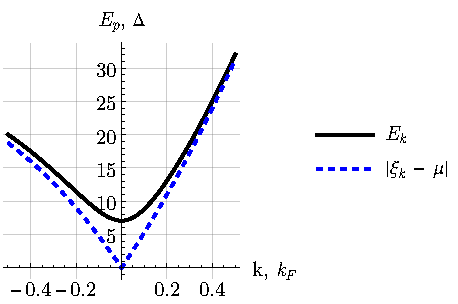
\includegraphics{imgs/MB132.pdf}
    \caption{The dispersion relation}
    \label{fig:131}
\end{figure}


\textbf{Ground state}. The BCS state
\begin{equation*}
	\gs = \prod_k \left(
		\sin \theta_k + \cos \theta_k c_{k \up}\D c_{-k \down}\D
	\right) \ket{0},
\end{equation*}
has zero Bogoliubov quasiparticles \textbf{(4)}:
\begin{align*}
	\gamma_{k \up} \gs &= \left(\sin \theta_k c_{k \up} - \cos \theta_k c_{-k \down}\D\right) \prod_k \left(
		\sin \theta_k + \cos \theta_k c_{k \up}\D c_{-k \down}\D
	\right) \ket{0} 
	\\&= \sin \theta_k c_{k \up} c_{k\up}\D c_{-k\down}\D \ket{0} - \cos \theta_k \sin \theta_k c_{-k\down}\D \ket{0} = 0,
\end{align*}
so $\gs$ is ground state of the mean field approximation of $H$. Actually the $\gs$ could be observed by
\begin{equation*}
	\gs \overset{\mathrm{n}}{=} \prod_{k} \gamma_{-k \down} \gamma_{k \down} \ket{0}.
\end{equation*}

In this state
\begin{equation*}
	E(\theta_k) = \bk{\text{gs}}[H]{\text{gs}} = \sum_k 2 \xi_k \cos^2 \theta_k + \frac{1}{4\Omega} \sum_{k k'} V_{kk'} \sin(2 \theta_k) \sin(2 \theta_{k'}),
\end{equation*}
and we could find $\theta_k$ just by minimizing the energy
\begin{equation*}
	\frac{\partial }{\partial \theta_q} E(\theta_k) = \frac{1}{\Omega}\cos(2 \theta_q) \sum_k V_{qk} \sin(2 \theta_k) - 2 \xi_q \sin(2 \theta_q) = 0.
\end{equation*}
Using this relation we could simplify expression \textbf{(5)}
\begin{equation*}
	\Delta_k = - \frac{1}{\Omega} \sum_{k'} V_{k k'} \langle c_{-k' \down} c_{k' \up} \rangle_{\text{gs}} = - \frac{1}{2\Omega}\sum_{k'}  V_{kk'} \sin(2 \theta_{k'}) = 
	- \frac{1}{\Omega} \sum_{k'} V_{k k'} \frac{\Delta_{k'}}{2 E_{k'}},
\end{equation*}
the zero temperature gap equation.








% and
% \begin{equation*}
% 		\hspace{5 mm} 
% 	\Leftarrow
% 	\hspace{5 mm} 
% 	\left\{c_{k \up}, c_{k' \up}\right\} = 0,
% 	 \ 
% 	\left\{c_{k \up}, c_{-k' \down}\right\} = 0,
% 	\ \ldots
% \end{equation*}




\newpage
\setcounter{section}{14}
\setcounter{subsection}{0}


\subsection{Specific heat of a BCS superconductor}
As we have shown in the previous exercise, in the mean field approximation the BCS Hamilto-
nian describes non-interacting fermionic Bogoliubov quasiparticles with dispersion $E_k$. Conse-
quently, their average occupation at inverse temperature $\beta$ is given by the Fermi-Dirac
distribution
\begin{equation*}
	\langle \hat{\gamma}_{k \sigma}\D \hat{\gamma}_{k \sigma}\rangle = f_k = \frac{1}{e^{\beta E_k(\beta)} + 1},
	\hspace{10 mm} 
	E_k = \sqrt{\xi_k^2 + \Delta_k^2(\beta)}.
\end{equation*}
Next we assume that $\sub{k}{B} = 1$.

\textbf{1. The specific heat}.  Starting from the expression
\begin{equation*}
	S = - 2 \sum_k \left(
		(1-f_k) \ln (1-f_k) + f_k \ln f_k
	\right),
\end{equation*}
for the entropy of a gas of non-interacting fermions, we could find 
\begin{equation*}
	C = T \frac{\partial S}{\partial T} \bigg|_V = - \beta \frac{\partial S}{\partial \beta}  = 2 \beta \sum_k \ln\left(\frac{f_k}{1-f_k}\right) \frac{\partial f_k}{\partial \beta}.
\end{equation*}
All that remains is to find
\begin{equation*}
	\frac{\partial f_k}{\partial \beta} = \left(\frac{1}{2E_k } \frac{d \Delta_k^2}{\beta} + \frac{E_k}{\beta}\right) \frac{\partial f_k}{\partial E_k},
\end{equation*}
thus
\begin{equation*}
	C = 2 \beta \sum_k \left(- \frac{\partial f_k}{\partial E_k} \right) \left(
		E_k^2 + \frac{\beta}{2} \frac{d \Delta+k^2}{d \beta} 
	\right).
\end{equation*}



\textbf{2. Nernst's theorem}. We can find low-temperature asymptotics to $C(\beta \to \infty)$
\begin{equation*}
	C = - 2 \beta V N(0) \int \frac{\partial f_k}{\partial E_k} \left(
		E_k^2 + \frac{\beta}{2} \frac{d \Delta^2}{d \beta} 
	\right) \d \xi.
\end{equation*}

For low temperatures we can neglect the temperature dependence for the $\Delta_k(\beta \to \infty) \approx 1.76 T_c$ and it is convenient to use the saddle-point method
\begin{equation*}
	C \approx 2 V N(0) \Delta^2 e^{-\beta \Delta} \int e^{- (\beta \xi)^2 / 2 \beta \Delta} \d (\beta \xi) = 2 \sqrt{2\pi} V N(0) (\beta \Delta)^{5/2} \frac{e^{-\beta \Delta}}{\beta},
\end{equation*}
which corresponds to the desired exponential decay. 
\begin{equation*}
	\frac{C}{C_n} \approx (\beta \Delta)^{5/2} e^{- \beta \Delta}.
\end{equation*}
So $C / C_n = 0.01$ at $\beta \Delta \approx 10$ or $T \approx 0.2 T_c$. 



\textbf{3.  The specific heat jump}. In a second order phase transition the jump in the specific heat just below $T_c$
\begin{equation*}
	\Delta C = - \beta^2 \frac{d \Delta^2}{d \beta}  \sum_k \frac{\partial f_k}{\partial E_k} \bigg|_{T_c-0} = 2V N(0) \beta^2 \frac{d \Delta^2}{d \beta} \bigg|_{T_c-0}  \int \frac{\partial f_k}{\partial E_k} \d \xi = \frac{8 \pi^2}{7 \zeta(3)} N(0) V T_c,
\end{equation*}
with $d \Delta^2 / d \beta|_{T_c-0} = 8 \pi^2 (T_c)^3 / (7 \zeta(3))$. The universal ratio is
\begin{equation*}
	\frac{\Delta C}{C_n(T_c)} = \frac{12}{7 \zeta(3)} \approx 1.43.
\end{equation*}


\textbf{4. Compressibility}. Consider now the BCS wavefunction at $T=0$. The BCS ground-state energy is then
\begin{equation*}
	\sub{\Omega}{g} = \sum_k \left(\xi_k - \sqrt{\xi_k^2 + |\Delta_k|^2} + \frac{|\Delta_k|^2}{2 E_k}\right),
	\hspace{10 mm} 
	\Delta_k = \Delta \theta(\hbar \sub{\omega}{D} - |\xi_k|),
\end{equation*}
with Debye temperature $T_D = \hbar \omega_D \gg \Delta$.  The zero-temperature isothermal compressibility
\begin{equation*}
	\kappa = - \frac{1}{V} \frac{\partial^2 \sub{\Omega}{g}}{\partial \mu^2}. 
\end{equation*}
More precisely, the difference from the ideal Fermi gas
\begin{equation*}
	\Delta \kappa = - \frac{1}{V} \frac{\partial^2 }{\partial \mu^2} \left(\sub{\Omega}{g}^\text{BCS} - \sub{\Omega}{g}^\text{FG}\right) =  - \frac{1}{2V} \frac{\partial^2 }{\partial \mu^2} \left( -N(\eF) \Delta^2 \right),
\end{equation*}
with $\Delta |_{T=0} \approx 2 \hbar \omega_D \exp\left(- \frac{1}{\alpha N(\eF)}\right)$. Due to we live in 3D $N(E) = \frac{\sqrt{2}}{\pi^2} \sub{m}{e}^{3/2} \sqrt{E}$.  Thus
\begin{equation*}
	\Delta \kappa = \frac{\Delta^2}{2V}\left(
		\frac{1}{\frac{\sqrt{2}}{\pi^2} \sub{m}{e}^{3/2} \alpha^2 \eF^{5/2} } - \frac{1}{2 \alpha \eF^2 } - \frac{\frac{\sqrt{2}}{\pi^2} \sub{m}{e}^{3/2}}{2 \eF^{3/2}}
	\right) > 0,
\end{equation*}
apparently because of Cooper pairs. 





\newpage
% % document's head

\begin{center}
    \LARGE \textsc{Название}
\end{center}

\hrule

\phantom{42}

\begin{flushright}
    \begin{tabular}{rr}
    % written by:
        % \textbf{Источник}: 
        % & \href{__ссылка__}{__название__} \\
        % & \\
        % \textbf{Лектор}: 
        % & _ФИО_ \\
        % & \\
        \textbf{Авторы заметок}: 
        & Хоружий Кирилл \\
        % & Примак Евгений \\
        & \\
    % date:
        \textbf{От}: &
        \textit{\today}\\
    \end{tabular}
\end{flushright}

\thispagestyle{empty}
\tableofcontents
\newpage



% % Lorem ipsum dolor sit amet, consectetur adipisicing elit, sed do eiusmod
% tempor incididunt ut labore et dolore magna aliqua. Ut enim ad minim veniam,
% quis nostrud exercitation ullamco laboris nisi ut aliquip ex ea commodo
% consequat. Duis aute irure dolor in reprehenderit in voluptate velit esse
% cillum dolore eu fugiat nulla pariatur. Excepteur sint occaecat cupidatat non
% proident, sunt in culpa qui officia deserunt mollit anim id est laborum.
% \begin{equation*}
% 	\ket{\psi} = \alpha_1 \raisebox{-6.3mm}{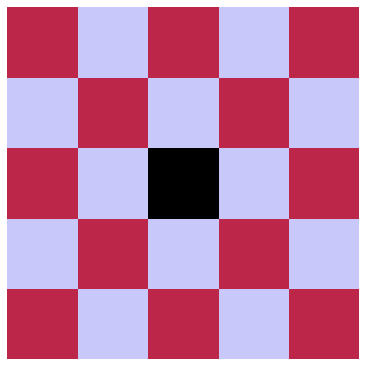
\includegraphics[width=0.08\textwidth]{s1.pdf}} + 
% 	\alpha_2 \raisebox{-6.3mm}{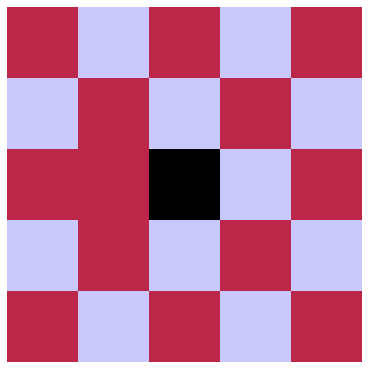
\includegraphics[width=0.08\textwidth]{s2.pdf}} + 
% 	\alpha_3 \raisebox{-6.3mm}{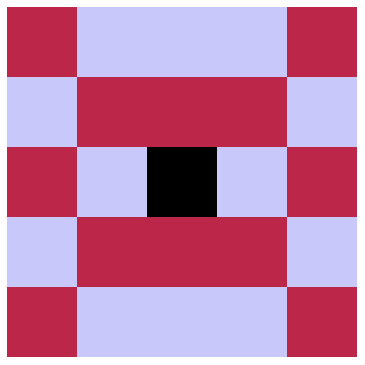
\includegraphics[width=0.08\textwidth]{s3.pdf}} + \ldots
% \end{equation*}

% \begin{equation*}
% 	\hat{H} = J \sum_{\langle i,j\rangle} \hat{S}_i \hat{S}_j - t \sum_{\langle i,j\rangle} \hat{c}_i\D \hat{c}_j
% \end{equation*}

% \begin{equation*}
% 	f(z) = \left\{\begin{aligned}
% 	    &1 - {\tilde{N}^0_{\text{pred}> z}}/{\tilde{N}^1_{\text{pred}< z}}, &z \geq \text{treshold} \\
% 	    &{\tilde{N}^1_{\text{pred}< z}}/{\tilde{N}^0_{\text{pred}> z}}-1, &z < \text{treshold} \\
% 	\end{aligned}\right.
% \end{equation*}


% \begin{equation*}
% 	f(z) = \tilde{N}^1_{\text{pred}< z}
% \end{equation*}


%  \begin{equation*}
%  	\hat{H} = - \sum_{\langle i,j\rangle} \hat{c}_i\D \hat{c}_j
%  \end{equation*}

%  \begin{equation*}
%  	g_2(r) = \langle \hat{c}_{\vc{j}}\D \hat{c}_{\vc{j}+\vc{r}}\D \hat{c}_{\vc{j}+\vc{r}}\hat{c}_{\vc{j}}\rangle_{\vc{j}}
%  \end{equation*}

%  \begin{equation*}
%  	\sub{\hat{H}}{FH} = - t \sum_{\langle i,j\rangle, \sigma} \hat{c}_{i \sigma}\D \hat{c}_{j \sigma} + U \sum_j \hat{n}_{j \uparrow} \hat{n}_{j \downarrow} + \sum_{j, \sigma} (V_j - \mu)\hat{n}_{j, \sigma}
%  \end{equation*}

%  \begin{equation*}
%  	{\hat{H}}_{tJ} = - t \sum_{\langle i,j\rangle, \sigma} \hat{c}_{i \sigma}\D \hat{c}_{j \sigma} + J \sum_{\langle i,j\rangle}\left(
%  		\hat{S}_i \hat{S}_j - \tfrac{1}{4} n_i n_j
%  	\right) + O(t^3 / U^2)
%  \end{equation*}

%  \begin{equation*}
%  	\langle \hat{O}\rangle(T) = \tfrac{1}{Z}\sum_j e^{- E_j / T} \bk{\psi_j}[\hat{O}]{\psi_j}
%  \end{equation*}

% \begin{equation*}
% {\hat{H}}_{tJ} = - t \sum_{\langle i,j\rangle, \sigma} \hat{c}_{i \sigma}\D \hat{c}_{j \sigma} + J \sum_{\langle i,j\rangle}
% 	\hat{S}_i \hat{S}_j
% \end{equation*}

% Stern-Gerlach: $F = \mu_z  \cdot \tfrac{\partial B}{\partial z} $



% \begin{equation*}
% 	\begin{pmatrix}
% 		\text{cost}_1 \\ \ldots \\ \text{cost}_n
% 	\end{pmatrix} \to \begin{pmatrix}
% 		w_1 \cdot \text{cost}_1 \\ \ldots \\ w_n \cdot  \text{cost}_n
% 	\end{pmatrix} 
% \end{equation*}



\setcounter{section}{1}
\subsection{Quantum State Tomography}

\begin{enumerate}[label=(\alph*)]
	\item 
Density matrix could be decomposed as 
\begin{equation*}
	\hat{\rho} = \frac{1}{2^N} \sum_{\{\alpha_j\}} C_{\alpha_1 \ldots \alpha_N} \hat{\sigma}_{\alpha_1} \otimes \ldots \otimes \hat{\sigma}_{\alpha_N},
\end{equation*}
with Pauli matrix $\hat{\sigma}_{j}$ and $\alpha = 0,1,2,3$
\begin{equation*}
 	\hat{\sigma}_0 = \begin{pmatrix}
 	    1 & 0 \\
 	    0 & 1 \\
 	\end{pmatrix},
 	\hspace{5 mm}
 	\hat{\sigma}_1 = \begin{pmatrix}
 	    0 & 1 \\
 	    1 & 0 \\
 	\end{pmatrix},
 	\hspace{5 mm} 
 	\hat{\sigma}_2 = \begin{pmatrix}
 	    0 & -i \\
 	    i & 0 \\
 	\end{pmatrix},
 	\hspace{5 mm} 
 	\hat{\sigma}_z = \begin{pmatrix}
 	    1 & 0 \\
 	    0 & -1 \\
 	\end{pmatrix}.
\end{equation*} 
Coefficients $C_{\alpha_1 \ldots \alpha_N}$ could be measured using $\hat{\sigma}_j^2 = \hat{\sigma}_0$
\begin{equation*}
	C_{\alpha_1 \ldots \alpha_N} = \tr \left(
		\hat{\rho} \  \hat{\sigma}_{\alpha_1} \otimes \ldots \otimes \hat{\sigma}_{\alpha_N}
	\right),
\end{equation*}
so we need $4^{N}-1$ measurements (remembering $\tr \rho = 1$). Doing finite number of shots we measure not average values by themselves, but their estemations, so we could observe not normalized states. For 2-qubit system a complete set of measurement operators is
\begin{equation*}
	\{\sigma_{\alpha_1} \otimes \sigma_{\alpha_2}\},
\end{equation*}
except $\alpha_1 = \alpha_2 = 0$.
	\item The Bloch vector can be extracted as
\begin{equation*}
	\ket{\psi} = \begin{pmatrix}
		\cos \theta /2 \\
		e^{i \varphi} \sin \theta/2
	\end{pmatrix},
	\hspace{0.5cm} \Rightarrow \hspace{0.5cm}
	\hat{\rho} = \kb{\psi}{\psi} = \frac{1}{2}\begin{pmatrix}
	    1+\cos \theta & e^{-i \varphi} \sin \theta \\
	    e^{i \varphi} \sin \theta & 1-\cos(\theta) \\
	\end{pmatrix},
\end{equation*}
what could be expand as
\begin{equation*}
	\hat{\rho} = \tfrac{1}{2} \hat{\sigma}_0 + \tfrac{1}{2} \sin \theta \cos \varphi \ \hat{\sigma}_x + \tfrac{1}{2}\sin \theta \sin \varphi\ \hat{\sigma}_y + \tfrac{1}{2}\cos \theta \ \hat{\sigma}_z.
\end{equation*}

\end{enumerate}


\subsection{Semi-Classical Light–Matter Interaction}

We have basic light-atom interaction
\begin{equation*}
	\hat{H} = \hat{H}_0 + \hat{V}
	,
	\hspace{10 mm} 
	\hat{H}_0 = - \frac{\hbar \omega}{2} \hat{\sigma}_z,
	\hspace{5 mm} 
	\hat{V}(t) = - \hbar \Omega \cos(\omega_L t) \hat{\sigma}_x,
\end{equation*}
with Rabi frequency $\Omega = d E_0 / \hbar$.

\begin{enumerate}[label=(\alph*)]
	\item Using that $\exp \diag (a_j) = \diag(e^{a_j})$ we could simplify
\begin{equation*}
	e^{- i \theta \hat{\sigma}_z} \hat{\sigma}_x e^{i \theta \hat{\sigma}_z} = 
	\begin{pmatrix}
	    e^{-i \theta} & 0 \\
	    0 & e^{i  \theta} \\
	\end{pmatrix} \begin{pmatrix}
	    0 & 1 \\
	    1 & 0 \\
	\end{pmatrix}
	\begin{pmatrix}
	    e^{i \theta} & 0 \\
	    0 & e^{-i  \theta} \\
	\end{pmatrix}
	=
	\cos(2\theta) \hat{\sigma}_x + \sin(2\theta) \hat{\sigma}_y.
\end{equation*}
	\item Using unitary tranform $\hat{U} = \exp\left(
	- \frac{i}{2} \omega_L t \hat{\sigma}_z
\right)$ we could substitute $\ket{\psi} = \hat{U}\D |\tilde{\psi}\rangle$ and find new $\sub{H}{I} = U H U\D - i \hbar U \partial_t U\D$:
\begin{equation*}
	\sub{\hat{H}}{I} = - \frac{\hbar}{2} \delta \begin{pmatrix}
	    1 & 0 \\
	    0 & -1 \\
	\end{pmatrix}
	 - \frac{\hbar}{2} \Omega \begin{pmatrix}
	     0 & 1 \\
	     1 & 0 \\
	 \end{pmatrix}
	 \grey{- \frac{\hbar}{2} \Omega \begin{pmatrix}
	     0 & e^{-2 i \omega_L t} \\
	     e^{2 i \omega_L t} & 0 \\
	 \end{pmatrix} },
\end{equation*}
with $\delta = \omega - \omega_L$.



	\item We can just throw away the gray term.
	\item Consider $\delta=0$, than with $\ket{\psi(0)} = \ket{e}$ we have
\begin{equation*}
	\ket{\psi(t)} = \left(i \sin(\tfrac{\Omega}{2}t),\ \cos(\tfrac{\Omega}{2}t)\right)\T,
\end{equation*}
so that $\langle \hat{\sigma}_z\rangle$ oscillate with frequency $\Omega$.
	\item $\nu = \frac{2 e L E}{h} \approx 24\,$MHz and $T_{\pi/2} \sim 10\,$ns
	\item $\Omega = \sqrt{\frac{6\pi I c^2 \Gamma}{\hbar \omega_0^3} } \sim 0.6\,\text{ms}^{-1} \to 0.1\,$kHz and 
$T_{\pi/2} \sim 2\,$ms
	\item We could simply solve Lindblad equation
\begin{equation}
	i \hbar \partial_t \hat{\rho} = \left[\hat{H}, \hat{\rho}\right] + i \hbar \hat{L}(\hat{\rho}),
	\hspace{5 mm} 
	\hat{L}(\hat{\rho}) = -\Gamma \begin{pmatrix}
	    -\rho_{22} & \tfrac{1}{2}\rho_{12} \\
	    \tfrac{1}{2}\rho_{21}& \rho_{22} \\
	\end{pmatrix}.
	\label{leq}
\end{equation}
Considering that the detuning is zero we have evolution 
% \begin{equation*}
% 	\partial_t \hat{\rho} = \frac{1}{2}\left(
% \begin{array}{cc}
%  2 \Gamma  \rho _{22}+\rho _{12} \Omega -\rho _{21} \Omega  & -\rho _{12} (\Gamma +2 \delta )+\rho _{11} \Omega -\rho _{22} \Omega  \\
%  -\rho _{21} (\Gamma -2 \delta )+\rho _{11} (-\Omega )+\rho _{22} \Omega  & -2 \Gamma  \rho _{22}+\rho _{12} (-\Omega )+\rho _{21} \Omega  \\
% \end{array}
% \right).
% \end{equation*}
%  and introducing $$ we have
\begin{equation*}
	\partial_t \hat{\rho} = \Gamma \left(
\begin{array}{cc}
 \rho _{22} & -\tfrac{\rho _{12}}{2} \\
 -\tfrac{\rho _{21}}{2} & -\rho _{22} \\
\end{array}
\right) - \frac{i \Omega}{2} \left(
\begin{array}{cc}
 \rho _{12}-\rho _{21} & \rho _{11}-\rho _{22} \\
 \rho _{22}-\rho _{11} & \rho _{21}-\rho _{12} \\
\end{array}
\right).
\end{equation*}
Consider the behavior of the $\rho_{22}$
 % $w = \tr(\hat{\rho} \hat{\sigma}_z) = \rho_{11}-\rho_{22}$
  with $\alpha = \Omega / \Gamma \ll 1$
\begin{equation*}
	\rho_{22} = \alpha^2 - \alpha ^2 e^{-\Gamma t} \left(2 e^{\frac{1}{2}\Gamma  t}-1\right) + O(\alpha^4).
\end{equation*}
With $\alpha = \Gamma / \Omega \ll 1$ we will have Rabi oscillations, converging to the $\rho_{11} = \rho_{22} = 1/2$ with envelope $\sim e^{-\alpha t}$.
\end{enumerate}



\subsection{Driven System Dynamics and Rotating-Wave Approximation}

Consider $H_0 = - \frac{\hbar \omega}{2} \sigma_z$ with $V = \frac{\hbar\Omega}{2}\cos(\omega t) \sigma_z - \frac{\hbar\Omega}{2} \sin(\omega t) \sigma_y $ (black dashed line) and $\sub{V}{RWA} = \hbar \Omega \cos(\omega t) \sigma_x$ (\blue{blue} line) in resonant $(\omega=\omega_0)$ case (fig. \ref{fig:rwa}).

\begin{figure}[h]
    \centering
    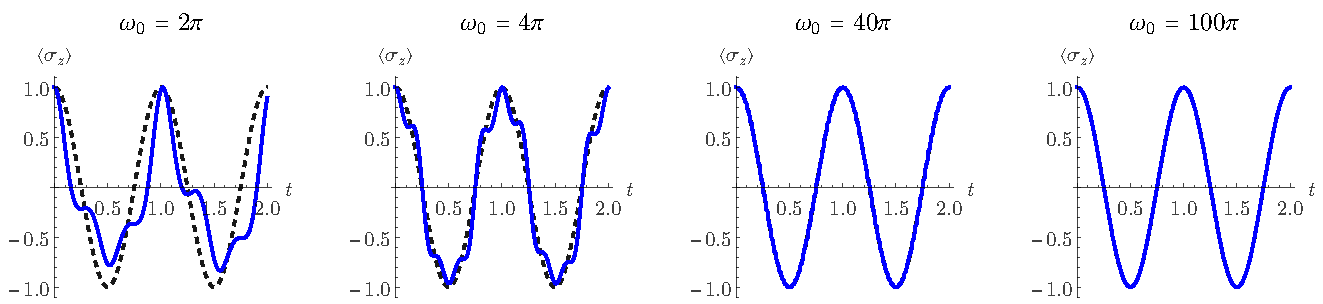
\includegraphics[width=1.0\textwidth]{figs/p23_1.pdf}
    \caption{Comparison of the exact solution (black) and the solution in the rotating wave approximation (blue).}
    \label{fig:rwa}
\end{figure}


We could find solution in general case $\delta \neq 0$ in RWA:
\begin{equation*}
	\langle \sigma_z\rangle(t) = \cos (\Omega_\delta t) + \frac{\delta ^2}{\delta ^2+\Omega ^2}(1-\cos (\Omega_\delta t )),
	\hspace{10 mm} 
	\Omega_\delta = \sqrt{\Omega^2 + \delta^2},
\end{equation*}
with general Rabi frequency $\Omega_\delta$. For different $\delta = 0, \Omega, 2 \Omega$ and $\Omega=2\pi$ we could compare different behaviour (fig. \ref{fig:rod}).

\begin{figure}[h]
    \centering
    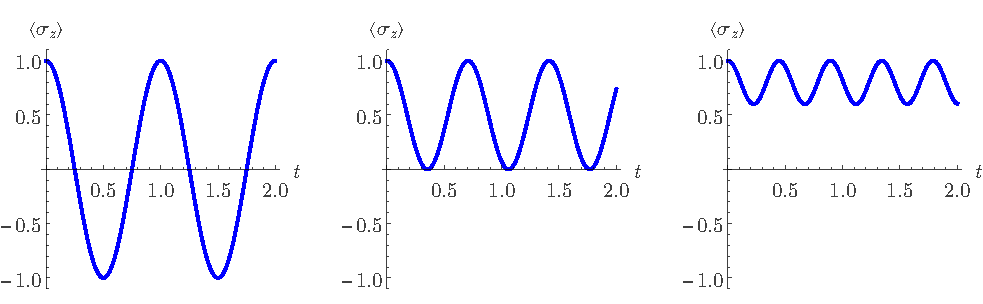
\includegraphics[width=0.75\textwidth]{figs/p23_2.pdf}
    \caption{Rabi oscillations at different detuning values}
    \label{fig:rod}
\end{figure}


\subsection{Dephasing and Decoherence in a TLS}

We could calculate $\langle \vc{\sigma}\rangle$, using  \eqref{leq}:
\begin{equation*}
	\rho(t) = \begin{pmatrix}
	    1-|\beta|^2 e^{- \Gamma_1 t} & \alpha \bar{\beta} e^{-\Gamma_2 t} \\
	    \bar{\alpha} \beta e^{- \Gamma_2 t} & |\beta|^2 e^{-\Gamma_1 t} \\
	\end{pmatrix},
	\hspace{0.5cm} \Rightarrow \hspace{0.5cm}
	\left.\begin{aligned}
	   \langle \sigma_x\rangle &= (\alpha \bar{\beta} + \bar{\alpha} \beta ) e^{- \Gamma_2 t}\\
	   \langle \sigma_y\rangle &= i(\alpha \bar{\beta} - \bar{\alpha} \beta ) e^{- \Gamma_2 t} \\
	   \langle \sigma_z\rangle &= 1 - 2 |\beta|^2 e^{-t \Gamma_1}
	\end{aligned}\right.
\end{equation*}
Substituting the initial state $\tfrac{1}{\sqrt{2}}\ket{0} + \tfrac{1}{\sqrt{2}}\ket{1}$
\begin{equation*}
	\langle \sigma_x\rangle =  e^{- \Gamma_2 t},
	\hspace{10 mm} 
	\langle \sigma_y\rangle = 0,
	\hspace{10 mm}
	\langle \sigma_z\rangle = 1 - e^{- \Gamma_1 t},
\end{equation*}
thus by measuring the various components we can find the $\Gamma_1$ and $\Gamma_2$, it's just exponential decay.




\phantom{42}

\vfill

\phantom{42} \hfill \textbf{\textit{\today, \ Khoruzhii Kirill}}
 % essay